	% Questo file definisce lo stile che verrà applicato
% ad ogni pagina di contenuto
\documentclass[a4paper,11pt]{article}

\usepackage{ifthen}
\usepackage[
 a4paper,
 top=2.5cm,
 bottom=2.5cm,
 left=1.5cm,
 right=1.5cm,
 head=30pt
]{geometry}
\usepackage[italian]{babel}
\usepackage[utf8x]{inputenc}
\usepackage[T1]{fontenc}
\usepackage{fancyhdr}
\usepackage[colorlinks=true, urlcolor=black, citecolor=black, linkcolor=black]{hyperref}
\usepackage{tabularx}
\usepackage{multirow}
\usepackage{booktabs}
\usepackage{color}
\usepackage[dvipsnames]{xcolor}
\usepackage{graphicx}
\usepackage{eurosym}
\usepackage{amsmath}
\usepackage{relsize}
\usepackage{placeins}
\usepackage{ltablex}
\usepackage{float}

\usepackage[multidot]{grffile}
\usepackage{xcolor,colortbl}
\definecolor{lightblue}{HTML}{56B4E6}
\definecolor{blue}{HTML}{2953A1}
\definecolor{darkblue}{HTML}{1E396E}
\usepackage{longtable}

\usepackage[toc,page]{appendix}
\renewcommand\appendixtocname{Appendice}
\renewcommand{\appendixpagename}{Appendice}

\newcommand\pagenumberingnoreset[1]{\gdef\thepage{\csname @#1\endcsname\c@page}}

% Cambia il font 
\renewcommand*\rmdefault{qhv}

% ***STILE PAGINA***
\pagestyle{fancy}
\fancyhf{}
\setlength{\headheight}{1cm} 
% No indentazione paragrafo
\setlength{\parindent}{0pt}

% ***INTESTAZIONE***
\newcommand\textline[4][t]{%
  \noindent\parbox[#1]{.333\textwidth}{\raisebox{-0.40\height}{#2}}%
  \parbox[#1]{.333\textwidth}{\centering #3}%
  \parbox[#1]{.333\textwidth}{\raggedleft #4}%
}

\lhead{
	\textline[t]{
\includegraphics[width=1cm, keepaspectratio=true]{../../../Template/Logo/Logo.png}}{\progettoShort}{\documento}
}

\renewcommand{\headrulewidth}{0.4pt}  %Linea sotto l'intestazione

% ***PIÈ DI PAGINA***
\lfoot{\textit{\gruppoLink}\\ \footnotesize{\email}}
\rfoot{\thepage} %per le prime pagine: mostra solo il numero romano
\cfoot{}
\renewcommand{\footrulewidth}{0.4pt}   %Linea sopra il piè di pagina


% Ridefinisce command \paragraph{} andando a capo ogni dopo la parola dentro le parentesi ed ha la possibiltà di enumerazione fino a n cifre modificando il numero dentro "secnumdepth"
\usepackage{titlesec}

\setcounter{secnumdepth}{7}
\setcounter{tocdepth}{7}


% Visualizza paragraph come una section
\titleformat{\paragraph}{\normalfont\normalsize\bfseries}{\theparagraph}{1em}{}
\titlespacing*{\paragraph}{0pt}{3.25ex plus 1ex minus .2ex}{1.5ex plus .2ex}

\titleformat{\subparagraph}{\normalfont\normalsize\bfseries}{\thesubparagraph}{1em}{}
\titlespacing*{\subparagraph}{0pt}{3.25ex plus 1ex minus .2ex}{1.5ex plus .2ex}

\makeatletter
\newcounter{subsubparagraph}[subparagraph]
\renewcommand\thesubsubparagraph{%
  \thesubparagraph.\@arabic\c@subsubparagraph}
\newcommand\subsubparagraph{%
  \@startsection{subsubparagraph}    % counter
    {6}                              % level
    {\parindent}                     % indent
    {3.25ex \@plus 1ex \@minus .2ex} % beforeskip
    {0.75em}                           % afterskip
    {\normalfont\normalsize\bfseries}}
\newcommand\l@subsubparagraph{\@dottedtocline{6}{13em}{5.5em}} %gestione dell'indice
\newcommand{\subsubparagraphmark}[1]{}
\makeatother

\makeatletter
\newcounter{subsubsubparagraph}[subsubparagraph]
\renewcommand\thesubsubsubparagraph{%
  \thesubsubparagraph.\@arabic\c@subsubsubparagraph}
\newcommand\subsubsubparagraph{%
  \@startsection{subsubsubparagraph}    % counter
    {7}                              % level
    {\parindent}                     % indent
    {3.25ex \@plus 1ex \@minus .2ex} % beforeskip
    {0.75em}                           % afterskip
    {\normalfont\normalsize\bfseries}}
\newcommand\l@subsubsubparagraph{\@dottedtocline{7}{16em}{6.5em}} %gestione dell'indice
\newcommand{\subsubsubparagraphmark}[1]{}
\makeatother

%Generali
\newcommand{\capitolato}{C5 - Monolith: An interactive bubble provider}
\newcommand{\progettoShort}{Monolith}
\newcommand{\progetto}{Monolith: An interactive bubble provider}
\newcommand{\gruppo}{NPE Developers}
\newcommand{\gruppoLink}{\href{https://gitlab.com/npe-developers}{NpeDevelopers}}
\newcommand{\email}{\href{mailto:npe.developers@gmail.com}{\textcolor{blue}{npe.developers@gmail.com}}}
\newcommand{\password}{NP3Devel0pers}
\newcommand{\myincludegraphics}[2][]{%
	\setbox0=\hbox{\phantom{X}}%
	\vtop{
		\hbox{\phantom{X}}
		\vskip-\ht0
		\hbox{\includegraphics[#1]{#2}}}
}




%Componenti del gruppo
\newcommand{\RM}{Riccardo Montagnin}
\newcommand{\MT}{Manuel Turetta}
\newcommand{\FB}{Francesco Bazzerla}
\newcommand{\SL}{Stefano Lia}
\newcommand{\LD}{Luca Dario}
\newcommand{\DC}{Diego Cavestro}
\newcommand{\ND}{Nicolò Dovico}

%Ruoli
\newcommand{\Pm}{Project Manager}
\newcommand{\Am}{Amministratore}
\newcommand{\AmP}{Amministratori}
\newcommand{\An}{Analista}
\newcommand{\AnP}{Analisti}
\newcommand{\Dev}{Sviluppatore}
\newcommand{\DevP}{Sviluppatori}
\newcommand{\Ver}{Verificatore}
\newcommand{\VerP}{Verificatori}
\newcommand{\Progr}{Programmatore}
\newcommand{\ProgrP}{Programmatori}
\newcommand{\Prog}{Progettista}
\newcommand{\ProgP}{Progettisti}



%Firme
\newcommand{\RMFirma}{\myincludegraphics[scale = 0.5]{../../../Template/Firme/RM.png}}
\newcommand{\MTFirma}{\myincludegraphics[scale = 0.5]{../../../Template/Firme/MT.png}}
\newcommand{\FBFirma}{\myincludegraphics[scale = 0.5]{../../../Template/Firme/FB.png}}
\newcommand{\SLFirma}{\myincludegraphics[scale = 0.5]{../../../Template/Firme/SL.png}}
\newcommand{\LDFirma}{\myincludegraphics[scale = 0.5]{../../../Template/Firme/LD.png}}
\newcommand{\DCFirma}{\myincludegraphics[scale = 0.5]{../../../Template/Firme/DC.png}}
\newcommand{\NDFirma}{\myincludegraphics[scale = 0.5]{../../../Template/Firme/ND.png}}

%Professori e proponente
\newcommand{\TV}{Prof. Tullio Vardanega}
\newcommand{\RC}{Prof. Riccardo Cardin}
\newcommand{\RB}{Red Babel}
\newcommand{\proponente}{Red Babel}

%Documenti
\newcommand{\Gl}{Glossario}
\newcommand{\glossario}{\textit{\Gl\_v.2.0.0.pdf}}
\newcommand{\AdR}{Analisi dei Requisiti}
\newcommand{\analisiDeiRequisiti}{\textit{\AdR\_v.2.0.0.pdf}}
\newcommand{\AdRvDue}{AnalisiDeiRequisiti}
\newcommand{\NdP}{Norme di Progetto}
\newcommand{\normeDiProgetto}{\textit{\NdP\_v.2.0.0.pdf}}
\newcommand{\PdP}{Piano di Progetto}
\newcommand{\pianoDiProgetto}{\textit{\PdP\_v.2.0.0.pdf}}
\newcommand{\SdF}{Studio di Fattibilità}
\newcommand{\studioDiFattibilita}{\textit{\SdF\_v.2.0.0.pdf}}
\newcommand{\PdQ}{Piano di Qualifica}
\newcommand{\pianoDiQualifica}{\textit{\PdQ\_v.2.0.0.pdf}}
\newcommand{\VI}{Verbale Interno}
\newcommand{\VE}{Verbale Esterno}
\newcommand{\ST}{Specifica Tecnica}
\newcommand{\MU}{Manuale Utente}
\newcommand{\DDP}{Definizione di Prodotto}

%Periodo di progetto
\newcommand{\ARM}{Analisi dei Requisiti di Massima}
\newcommand{\ARD}{Analisi dei Requisiti in Dettaglio}
\newcommand{\PA}{Progettazione Architetturale}
\newcommand{\PD}{Progettazione di Dettaglio}
\newcommand{\COD}{Codifica}
\newcommand{\VV}{Verifica e Testing Finale}

%Consegne
\newcommand{\RR}{Revisione dei Requisiti}
\newcommand{\RP}{Revisione di Progettazione}
\newcommand{\RQ}{Revisione di Qualifica}
\newcommand{\RA}{Revisione di Accettazione}


%Formattazione
\newcommand{\termine}[1]{\textit{#1}\small{$_G$}}
\newcommand{\link}[1]{\href{#1}{\textcolor{blue}{\texttt{#1}}}} 

% Testi ricorrenti
\newcommand{\scopoProdotto}{L'obiettivo di questo progetto è la realizzazione di un \termine{SDK} che permetta la creazione di bolle interattive, le quali, successivamente, verranno utilizzate all'interno dell'applicazione di messaggistica istantanea open source \termine{Rocket.chat}. \\
Dopo la realizzazione di tale \termine{SDK}, è proposto lo sviluppo di un'applicazione in grado di sfruttare l'\termine{SDK} per implementare un uso originale. L'applicazione scelta dal \termine{team} consiste nella bolla lista-spesa e nei suoi vari utilizzi all'interno della piattaforma \termine{Rocket.chat}.
}
\newcommand{\descrizioneGlossario}{Al fine di mantenere questo documento compatto e di facile lettura è stato realizzato un glossario esterno contenente tutte le definizioni dei termini che più comunemente verranno presentati al lettore.  
Tale glossario si ritrova all'interno del file \glossario, e contiene tutti e soli i termini che vengono marcati con una \textit{G} a pedice.
}
\newcommand{\riferimentiNormativi}{
	\begin{itemize}
		\item \textbf{Norme di Progetto}: \normeDiProgetto
		\item \textbf{\termine{Capitolato} d'appalto C5: Monolith - An Interactive bubble provider} \\
			  \link{http://www.math.unipd.it/~tullio/IS-1/2016/Progetto/C5.pdf}
	\end{itemize}
}

% Comandi per generare l'intro
\newcommand{\documento}{\AdR}
\newcommand{\versione}{2.0.0}
\newcommand{\redatori}{\DC\\ & \LD\\ & \RM}
\newcommand{\revisori}{\SL}
\newcommand{\dataApprovazione}{28 febbraio 2017}
\newcommand{\approvazione}{\ND}
\newcommand{\statoapprovazione}{Approvato}
\newcommand{\uso}{Esterno}
\newcommand{\destinatari}{\RB\\ & \TV\\ & \RC}

\newcommand{\sommario}{Il presente documento vuole esporre al committente l'analisi dei requisiti effettuata e le potenzialità del sistema software ideato al fine di soddisfare le richieste del capitolato \capitolato.".
}
\usepackage{graphicx}
\usepackage{placeins}
\usepackage{ltablex}
\usepackage{float}


\newcommand{\modifiche}{
3.0.0 & Approvazione del documento - Creare nuova versione del documento & \SL & \Pm & 07/05/2017 \\\midrule
2.1.0 & Verifica documento - Correzione errori & \LD & \Ver & 04/05/2017 \\\midrule
2.0.4 & Aggiunta la nota riguardante la forma del \MU\ di \progettoShort\ - In seguito a quanto deciso in data 03 maggio 2017 e riportato nell'apposito verbale & \ND & \Am & 04/05/2017 \\\midrule
	2.0.3 & Modificata la sezione delle metriche per la codifica - Aggiungere regole più precise per facilitare la stesura del codice & \ND & \Am & 28/03/2017 \\\midrule
2.0.2 & Aggiunte sezioni mancanti - Migliorare la profondità del documento come segnalato nella correzione in seguito alla \RP & \SL & \Am & 27/03/2017 \\
\midrule
2.0.1 & Riorganizzata la sezione degli strumenti - Aggiungere chiarezza su quale strumento sia usato per quale attività & \SL & \Am & 26/03/2017 \\
\midrule
2.0.0 & Approvazione del documento - Creare nuova versione del documento & \DC & \Pm & 04/03/2017 \\
\midrule 
1.1.0 & Verifica del documento - Correzioni errori & \LD & \Ver & 04/03/2017 \\
\midrule 
	1.0.2 & Aggiunta metriche - Aggiunta profondità come segnalato nella correzione in seguito alla \RR & \ND & \Am & 28/02/2017 \\
	\midrule
	1.0.1 & Aggiornamenti sezioni 3 e 4 - Aggiunta ampiezza come segnalato nella correzione in seguito alla \RR & \ND & \Am & 27/02/2017 \\
	\midrule
	1.0.0 & Approvazione - Creare la prima versione del documento & \SL & \Pm & 04/01/2016 \\
	\midrule
	0.4.0 & Verifica sottosezione 4.4 - Correzione errori & \RM & \Ver & 29/12/2016 \\\midrule
	0.3.1 & Stesura sottosezione 4.4 - Aggiunte norme sul processo di formazione & \DC & \Ver & 29/12/2016 \\\midrule
	0.3.0 & Verifica sezione 4 - Correzione errori & \RM &\Ver & 27/12/2016 \\\midrule
	0.2.0 & Verifica sezione 3 - Correzione errori & \RM & \Ver & 24/12/2016 \\\midrule
	0.1.0  & Verifica sezioni 1 e 2 - Correzioni errori & \RM & \Ver & 23/12/2016\\\midrule
    0.0.5 & Stesura sezione 4 - stabilire norme per il coordinamento e pianificazione & \DC & \Am & 21/12/2016 \\\midrule
    0.0.4 & Stesura sezione 2 - Definizione dei processi primari per il progetto & \LD & \Am & 20/12/2017 \\\midrule
    0.0.3 & Stesura sezione 1 e modifica del template - Introduzione al documento & \FB & \Am & 18/12/2016 \\\midrule
    0.0.2 & Stesura sezione 3 - Definizione dei processi di supporto  & \ND & \Am & 17/12/2016 \\\midrule
    0.0.1 & Creazione del template - Inizio documento & \SL & \Am & 15/12/2016 \\\midrule
}


\begin{document}

% Questo file contiene il layout della prima pagina
\pagenumbering{gobble}

\title{
\includegraphics[width=8cm, keepaspectratio=true]{../../../Template/Logo/Logo.png} \\
	\documento \\
	Versione \versione
}
\date{\dataApprovazione}

\maketitle

\begin{center}

\begin{tabular}{ r | l }
  \textbf{Ruolo} & \textbf{Componente} \\
  Redazione & \redatori \\
  Revisione & \revisori \\
  Approvazione & \approvazione \\
  \\
  Stato & \statoapprovazione \\
  Uso & \uso \\
  Destinatari & \destinatari
\end{tabular}
\end{center}

\begin{center}
\textbf{Sommario\\}
\sommario \\
\vspace{1.5cm}\email
\end{center}

\clearpage

\pagenumbering{arabic}
%Questo file si occupa di generare la tabella delle modifiche
\pagenumbering{Roman}

\begin{center}
    \Large{\textbf{Registro delle modifiche}}
    	\\\vspace{0.5cm}
    	\normalsize
    \begin{tabularx}{\textwidth}{cXXcc}
        \textbf{Versione} & \textbf{Modifica - Motivazione} & \textbf{Autore} & \textbf{Ruolo} & \textbf{Data} \\\toprule
        \modifiche
    \end{tabularx}
\end{center}

\newpage



\tableofcontents

\newpage

\setcounter{table}{0}
\listoftables

\newpage

\listoffigures

\newpage

\pagenumbering{arabic}


\section{Introduzione}
\subsection{Scopo del documento}
Questo documento vuole definire le strategie che il \termine{team} ha deciso di adottare per perseguire gli obiettivi di qualità di processo e di prodotto ricercati. A tal fine è necessaria una costante attività di verifica e validazione del lavoro svolto in modo da poter rilevare e correggere le anomalie che potrebbero nascere.

\subsection{Scopo del prodotto}
\scopoProdotto

\subsection{Glossario}
\descrizioneGlossario

\subsection{Riferimenti}
\subsubsection{Normativi}
\riferimentiNormativi

\subsubsection{Informativi}
\begin{itemize}
	\item \textbf{\AdR}: \analisiDeiRequisiti;
	\item \textbf{\PdP}: \pianoDiProgetto;
	\item \textbf{\textit{Slide} dell'insegnamento di Ingegneria del Software}: \\
		  \link{http://www.math.unipd.it/~tullio/IS-1/2016/}
	\item \textbf{\textit{Standard} ISO/IEC 9126}: Product quality \\
	 	  \link{https://en.wikipedia.org/wiki/ISO/IEC\_9126}
	\item \textbf{\textit{Standard} tecnici ISO/IEC 15504}: Software process assessment \\
		  \link{https://en.wikipedia.org/wiki/ISO/IEC\_15504}
	\item \textbf{Ciclo di Deming (\termine{PDCA})}: Miglioramento dei processi \\
		  \link{https://en.wikipedia.org/wiki/PDCA}
\end{itemize}

\newpage
\section{Descrizione generale}
\subsection{Obiettivo del Prodotto}
\scopoProdotto

\subsection{Funzioni del prodotto}
Un qualsiasi utente dell'\termine{SDK} potrà creare e personalizzare le bolle messe a disposizione all'interno dell'\termine{SDK} e, successivamente, le visualizzerà come se fossero dei messaggi normali. Ogni \termine{bolla}, inoltre, avrà un suo uso e funzionalità specifiche, che verranno illustrate all'utente non appena egli deciderà di utilizzarla.

\subsection{Caratteristiche degli utenti}
Non sono richieste competenze particolari per poter usufruire dell'applicazione associata al progetto, che deve risultare quindi accessibile ad un ampia categoria di utenti. L'interfaccia dovrà quindi essere il più semplice e intuitiva possibile e favorirne un facile utilizzo. \\
Per quanto riguarda l'\termine{SDK}, esso verrà sviluppato con lo scopo di risultare quanto più comprensibile possibile, al fine di facilitarne l'utilizzo. \\
Verrà inoltre fornito un \MU\ per facilitare la comprensione dell'utilizzo di entrambi i prodotti realizzati per questo capitolato.

\subsection{Piattaforma di esecuzione} 
La piattaforma di esecuzione dell'applicazione che sfrutta l'\termine{SDK} è esclusivamente la \termine{web chat} \termine{Rocket.chat}.

\subsection{Vincoli generali}
Gli utenti che vogliono utilizzare l'applicazione creata dal gruppo \gruppo\ dovranno accedere all'istanza del server fornita dal gruppo stesso. \\
Per poter invece utilizzare l'\termine{SDK}, lo \termine{sviluppatore} dovrà includere il pacchetto \textit{Monolith} tramite il \termine{package manager} \termine{Atmosphere}. 

\newpage
\section{Casi d'uso}
In questa sezione vengono elencati i casi d'uso rilevati dall'analisi del capitolato \capitolato\ durante le riunioni con \RB\ e riguardanti l'\termine{SDK} e l'applicazione \termine{demo}. Questa consiste in una bolla lista della spesa condivisa, nella quale gli utenti sono divisi secondo le capacità di interazione con la lista.

Ogni caso d'uso è identificato dal seguente formalismo:
\begin{center}
	UC[\texttt{codice}]
\end{center}
dove \texttt{codice} è il codice gerarchico, numerico ed univoco, per identificare ogni caso d'uso.

\subsection{Attori}
Di seguito è riportato il diagramma \termine{UML} che descrive la gerarchia degli attori.

\label{Attori}
\begin{figure}[ht]
	\centering
	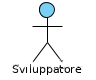
\includegraphics[scale=0.5]{Usecases/img/Attori.png}
	\caption{Attori dell'applicazione}
\end{figure}

\subsubsection{Sviluppatore}
Viene definito \termine{sviluppatore} una qualsiasi persona che abbia accesso diretto all'\termine{SDK} e ai suoi contenuti, e che lo utilizzerà al fine di creare una applicazione che ne sfrutti le caratteristiche.

\subsubsection{Utente}
Viene definito utente una qualsiasi persona che utilizzi la bolla lista della spesa.
\subsubsection{Utente esterno}
Un utente esterno è una raffinazione del concetto di utente, e consiste in un utente che ha ricevuto una bolla lista della spesa tramite inoltro, e che quindi può solamente visualizzare la lista ma non interagirci in alcun modo.
\subsubsection{Utente senza permessi}
Un utente senza permessi è una raffinazione del concetto di utente, e consiste in un utente che ha ricevuto la bolla lista della spesa tramite pubblicazione, e che quindi può spuntare i prodotti di quest'ultima. Non può, però, modificare i prodotti presenti all'interno della lista.
\subsubsection{Utente con permessi}
Un utente con permessi è un utente che ha ricevuto la lista tramite pubblicazione. Può quindi spuntarne i prodotti e inoltre ha ricevuto, dal creatore della lista, l'autorizzazione a modificare,aggiungere o rimuovere prodotti dalla lista stessa.
\subsubsection{Creatore della lista}
Il creatore della lista gode di tutte le proprietà dell'utente con permessi, ma in aggiunta può decidere se mandare una bolla lista tramite inoltro o tramite pubblicazione e concedere permessi di modifica della lista agli utenti che ha invitato tramite pubblicazione, decidendo o meno la partecipazione attiva degli altri utenti.



\FloatBarrier
\subsection{Caso d'uso UC 0: \progetto (SDK)}
\label{Caso d'uso UC 0: \progetto (SDK)}
\begin{figure}[ht]
	\centering
	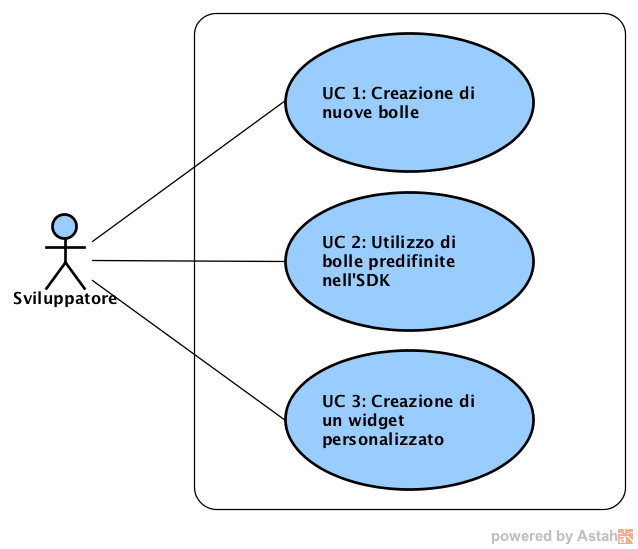
\includegraphics[scale=0.80]{Usecases/img/Monolith.png}
	\caption{Caso d'uso UC 0: \progetto(SDK)}
\end{figure}

\FloatBarrier
\begin{itemize}
\item \textbf{Attori:} Sviluppatore.
\item \textbf{Descrizione:} Tramite l'\termine{SDK} lo sviluppatore vuole:
	\begin{itemize}
	\item{Creare una nuova bolla utilizzando i widget dell'\termine{SDK}.}
	\item{Utilizzare una bolla predefinita.}
	\item{Creare un nuovo widget.}
	\end{itemize}
\item \textbf{Precondizione:} Lo sviluppatore ha accesso all'\termine{SDK}.
\item \textbf{Postcondizione:} Lo sviluppatore ha creato del codice eseguibile.
\item \textbf{Scenario Principale:}
	\begin{itemize}
	\item{Creazione di nuove bolle utilizzando i widget dell'\termine{SDK} (UC 1).}
	\item{Utilizzo di bolle predefinite nell'\termine{SDK} (UC 2).}
	\item{Creazione di un widget personalizzato (UC 3).}
	\end{itemize}
\end{itemize}
\newpage
\subsection{Caso d'uso UC 1: Creazione di nuove bolle}
\label{Caso d'uso UC 1: Creazione di nuove bolle}
\begin{figure}[ht]
	\centering
	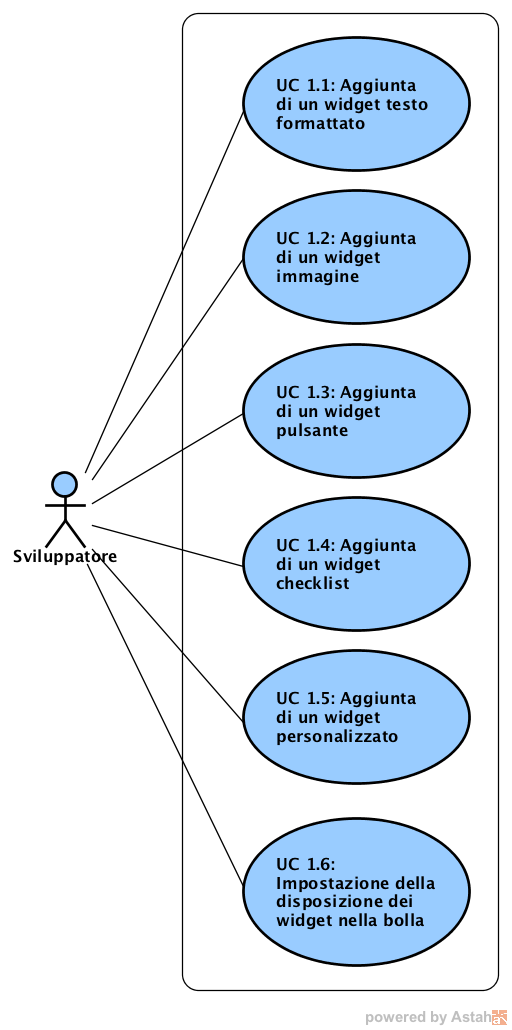
\includegraphics[scale=0.65]{Usecases/img/UC1.png}
	\caption{Caso d'uso UC 1: Creazione di nuove bolle}
\end{figure}

\FloatBarrier
\begin{itemize}
\item \textbf{Attori:} Sviluppatore;
\item \textbf{Descrizione:} Tramite l'\termine{SDK} lo sviluppatore vuole:
	\begin{itemize}
	\item{Aggiunta di un widget testo formattato a una bolla.} 
	\item{Aggiunta di un widget immagine a una bolla.}
	\item{Aggiunta di un widget bottone a una bolla.}
	\item{Aggiunta di un widget checklist a una bolla.}
	\item{Aggiunta di un widget personalizzato a una bolla.}
	\item{Impostare la disposizione dei widget nella bolla.}
	\end{itemize} 
\item \textbf{Precondizione:} Lo sviluppatore ha accesso all'\termine{SDK}.
\item \textbf{Postcondizione:} Lo sviluppatore ha creato del codice eseguibile. 
\item \textbf{Scenario principale:}
	\begin{itemize}
	\item{Lo sviluppatore vuole aggiungere a una bolla un widget testo formattato (UC 1.1).}
	\item{Lo sviluppatore vuole aggiungere a una bolla un widget immagine (UC 1.2).}
	\item{Lo sviluppatore vuole aggiungere a una bolla un widget pulsante (UC 1.3).}
	\item{Lo sviluppatore vuole aggiungere a una bolla un widget checklist (UC 1.4).}
	\item{Lo sviluppatore vuole aggiungere a una bolla un widget personalizzato (UC 1.5).}
	\item{Lo sviluppatore vuole impostare la disposizione dei wiget nella bolla (UC 1.6).}
	\end{itemize}
\end{itemize}
\subsubsection{Caso d'uso UC 1.1: Utilizzo di un widget testo formattato}
\label{Caso d'uso UC 1.1: Utilizzo di un widget testo formattato}

\begin{figure}[ht]
\centering
	\includegraphics[scale=0.6]{Usecases/img/{UC1.1}.png}
	\caption{Caso d'uso UC 1.1: Aggiunta di un widget testo formattato}
\end{figure}

\FloatBarrier
\begin{itemize}
\item\textbf{Attori}: Sviluppatore.
\item\textbf{Descrizione}: Lo sviluppatore vuole aggiungere a una bolla un widget testo formattato.
\item\textbf{Precondizione}: Lo sviluppatore ha accesso all'\termine{SDK}.
\item\textbf{Postcondizione}: Lo sviluppatore ha creato del codice eseguibile che permette di aggiungere a una bolla un widget testo formattato.
\item\textbf{Scenario principale}:
	\begin{itemize}
		\item Lo sviluppatore vuole scegliere la grandezza del font del testo (UC 1.1.1).
		\item Lo sviluppatore vuole impostare parte del testo in corsivo (UC 1.1.3).
		\item Lo sviluppatore vuole aggiungere un link cliccabile (UC 1.1.4).
		\item Lo sviluppatore vuole impostare parte del testo in grassetto (UC 1.1.7).
		\item Lo sviluppatore vuole impostare un colore a parte del testo (UC 1.1.8).
		\item Lo sviluppatore vuole aggiungere del testo alla bolla (1.1.10)
	\end{itemize}
	
\item\textbf{Scenario alternativo}
	\begin{itemize}
		\item Lo sviluppatore non inserisce la grandezza del font oppure la inserisce in modo non valido(UC 1.1.2).
		\item Lo sviluppatore non inserisce il colore del link cliccabile oppure lo inserisce in modo non valido(UC 1.1.6).
		\item Lo sviluppatore non imposta il colore del testo della bolla oppure lo inserisce in modo non valido(UC 1.1.9).
		\item Lo sviluppatore non inserisce del testo oppure lo inserisce in modo non valido(UC 1.1.11).
		
	\end{itemize}

\end{itemize}

\paragraph{Caso d'uso 1.1.1: Scelta della grandezza del font}
\begin{itemize}
\item\textbf{Attori}: Sviluppatore.
\item\textbf{Descrizione}: Lo sviluppatore vuole scegliere la grandezza del font della proprio widget.
\item\textbf{Precondizione}: Lo sviluppatore utilizza un widget testo formattato e vuole impostare la grandezza del font.
\item\textbf{Postcondizione}: Lo sviluppatore ha creato del codice eseguibile che permette di creare un widget testo formattato contenente del testo con la grandezza del font impostata.
\item\textbf{Estensioni:}
	\begin{itemize}
		\item Impostazione della grandezza del font a default (UC 1.1.2).
	\end{itemize}
\item\textbf{Scenario principale}: Lo sviluppatore utilizza un widget testo formattato e vuole impostare la grandezza del font. 
\item\textbf{Scenari alternativi}: La grandezza del font viene impostata a default (UC 1.1.2).
\end{itemize}
\paragraph{Caso d'uso 1.1.2: Impostazione della grandezza del font a default}
\begin{itemize}
\item\textbf{Attori}: Sviluppatore.
\item\textbf{Descrizione}: Se lo sviluppatore non ha impostato la grandezza del font o lo ha impostato con una grandezza non valida il font viene configurato ad un valore di default.
\item\textbf{Precondizione}: Lo sviluppatore ha impostato una grandezza del font non valida alla bolla di tipo testo formattato o non ha impostato alcuna grandezza al font.
\item\textbf{Postcondizione}: Lo sviluppatore ha creato del codice eseguibile cSe lo sviluppatore non ha impostato il colore del link o lo ha impostato con una colore non valido il link viene impostato con il colore blu.he permette di creare una bolla di testo formattato contenente del testo con una grandezza del font impostata a default.
\end{itemize}
\paragraph{Caso d'uso 1.1.3: Visualizzazione di parte del testo in corsivo}
\begin{itemize}
\item\textbf{Attori}: Sviluppatore.
\item\textbf{Descrizione}: Lo sviluppatore vuole impostare in corsivo parte del testo di una bolla di tipo testo formattato.
\item\textbf{Precondizione}: Lo sviluppatore utilizza una bolla di testo formattato e vuole impostare parte del testo in corsivo.
\item\textbf{Postcondizione}: Lo sviluppatore ha creato codice eseguibile per creare una bolla di tipo testo formattato che contiene parte del testo in corsivo.
\end{itemize}
\paragraph{Caso d'uso 1.1.4: Aggiunta di link cliccabili}
\begin{itemize}
\item\textbf{Attori}: Sviluppatore.
\item\textbf{Descrizione}: Lo sviluppatore vuole aggiungere un link cliccabile ad una bolla di tipo testo formattato che porti l'utente a visualizzare una pagina web esterna alla bolla stessa.
\item\textbf{Precondizione}: Lo sviluppatore utilizza una bolla di testo formattato e vuole aggiungere un link cliccabile.
\item\textbf{Postcondizione}: Lo sviluppatore ha creato codice eseguibile che permette di creare una bolla di testo formattato che contiene un link cliccabile.

\item\textbf{Inclusioni:}
	\begin{itemize}
		\item Lo sviluppatore seleziona il colore del link cliccabile (UC 1.1.5).
	\end{itemize}

	
\end{itemize}
\paragraph{Caso d'uso 1.1.5: Impostazione del colore del link}
\begin{itemize}
\item\textbf{Attori}: Sviluppatore.
\item\textbf{Descrizione}: Lo sviluppatore vuole selezionare il colore di un link cliccabile prima che esso venga cliccato da parte dell'utente finale della bolla.
\item\textbf{Precondizione}: Lo sviluppatore utilizza una bolla di tipo testo formattato con presente al suo interno un link cliccabile di cui vuole impostare il colore.
\item\textbf{Postcondizione}: Lo sviluppatore ha creato codice eseguibile che permette di creare una bolla di testo formattato contenente un link cliccabile che viene visualizzato con il colore impostato.

\item\textbf{Estensioni:}
	\begin{itemize}
		\item Impostazione del colore del link a blu (UC 1.1.6).
	\end{itemize}
\end{itemize}
\paragraph{Caso d'uso 1.1.6: Impostazione del colore del link a blu}
\begin{itemize}
\item\textbf{Attori}: Sviluppatore.
\item\textbf{Descrizione}: Se lo sviluppatore non ha impostato il colore del link o lo ha impostato con una colore non valido il link viene impostato con il colore blu.
\item\textbf{Precondizione}: Lo sviluppatore ha impostato un colore non valido al link di una bolla di tipo testo formattato o non ha impostato alcun colore al link.
\item\textbf{Postcondizione}: Il testo del link cliccabile viene impostato a blu.
\end{itemize}
\paragraph{Caso d'uso 1.1.7: Visualizzazione di parte del testo in grassetto}
\begin{itemize}
\item\textbf{Attori}: Sviluppatore.
\item\textbf{Descrizione}: Lo sviluppatore vuole impostare in grassetto parte del testo di un widget testo formattato.
\item\textbf{Precondizione}: Lo sviluppatore utilizza un widget testo formattato e vuole impostare parte del testo in grassetto.
\item\textbf{Postcondizione}: Lo sviluppatore ha creato codice eseguibile che permette di creare un widget testo formattato contenente parte del testo in grassetto.
\item\textbf{Scenario principale}: Lo sviluppatore vuole impostare in grassetto parte del testo di un widget testo formattato.
\end{itemize}
\paragraph{Caso d'uso 1.1.8: Impostazione del colore di parte del testo}
\begin{itemize}
\item\textbf{Attori}: Sviluppatore.
\item\textbf{Descrizione}: Lo sviluppatore vuole impostare un colore a parte del testo di una bolla di testo formattato.
\item\textbf{Precondizione}: Lo sviluppatore utilizza una bolla di tipo testo formattato e vuole impostare un colore colore personalizzato al testo.
\item\textbf{Postcondizione}: Lo sviluppatore ha creato codice eseguibile che permette di creare una bolla di testo formattato contenente una parte del testo visualizzato con il colore impostato.
\item\textbf{Estensioni:}
	\begin{itemize}
		\item Visualizzazione di un messaggio d'errore (UC 1.1.9).
		\end{itemize}

\end{itemize}
\paragraph{Caso d'uso 1.1.9 Impostazione del colore del testo a default}
\begin{itemize}
\item\textbf{Attori}: Sviluppatore.
\item\textbf{Descrizione}: Se lo sviluppatore non imposta il colore del font o lo imposta con un colore non valido il colore del font viene configurato ad un valore di default.
\item\textbf{Precondizione}: Lo sviluppatore vuole impostare un colore al testo di un widget tipo testo formattato non valido o non ha impostato alcun colore al testo.
\item\textbf{Postcondizione}: Il colore del testo viene impostato ad un valore di default.
\item\textbf{Scenario principale}: Lo sviluppatore ha commesso un errore nell'impostazione del colore del testo, perciò questo viene impostato a default.
\end{itemize}
\paragraph{Caso d'uso 1.1.10: Aggiunta di testo al widget}
\begin{itemize}
\item\textbf{Attori}: Sviluppatore.
\item\textbf{Descrizione}: Lo sviluppatore vuole aggiungere del testo a un widget testo formattato già esistente.
\item\textbf{Precondizione}: Lo sviluppatore vuole utilizzare un widget testo formattato e vuole aggiungere del testo a tale widget.
\item\textbf{Postcondizione}: Lo sviluppatore ha creato codice eseguibile che permette di aggiungere del testo ad un widget testo formattato già esistente.
\item\textbf{Estensioni:}
	\begin{itemize}
		\item Visualizzazione di un messaggio d'errore (UC 1.1.11).
		\end{itemize}
\item\textbf{Scenario principale}: Lo sviluppatore vuole aggiungere del testo a un widget testo formattato già esistente.
\item\textbf{Scenari alternativi}: 
	\begin{itemize}
	\item Viene visualizzato un messaggio d'errore (UC 1.1.11).
	\end{itemize}
\end{itemize}
\paragraph{Caso d'uso 1.1.11 Visualizzazione messaggio d'errore}
\begin{itemize}
\item\textbf{Attori}: Sviluppatore.
\item\textbf{Descrizione}: Lo sviluppatore viene avvisato con un messaggio d'errore dell'aggiunta in modo errato di ulteriore testo nel widget testo formattato.
\item\textbf{Precondizione}: Lo sviluppatore ha aggiunto in modo errato del testo in un widget testo formattato.
\item\textbf{Postcondizione}: Viene visualizzato un messaggio d'errore.
\item\textbf{Scenario principale}: Lo sviluppatore visualizza un messaggio d'errore.
\end{itemize}
\subsubsection{Caso d'uso UC 1.2: Utilizzo di una bolla di tipo bottone}
\label{Caso d'uso UC 1.2: Utilizzo di una bolla di tipo bottone}
\begin{figure}[ht]
	\centering
	\includegraphics[scale=0.80]{Usecases/img/{UC1.2}.png}
	\caption{Caso d'uso UC 1.2: Utilizzo di una bolla di tipo bottone}
\end{figure}
\FloatBarrier
\begin{itemize}
\item\textbf{Attori}: Sviluppatore.
\item\textbf{Descrizione}: Lo sviluppatore vuole utilizzare una bolla di tipo bottone.
\item\textbf{Precondizione}: Lo sviluppatore vuole utilizzare una bolla di tipo bottone.
\item\textbf{Postcondizione}: Lo sviluppatore crea codice eseguibile per creare una bolla di tipo bottone.
\item\textbf{Scenario principale}:
	\begin{itemize}
		\item Lo sviluppatore vuole utilizzare una bolla di tipo \termine{bottone semplice}(UC 1.2.1).
		\item Lo sviluppatore vuole utilizzare una bolla di tipo \termine{checkbutton}(UC 1.2.2).
		\item Lo sviluppatore vuole impostare una reazione ad un evento del bottone(UC 1.2.3).
	\end{itemize}

\end{itemize}


\paragraph{Caso d'uso UC 1.2.1: Utilizzo di una bolla di tipo bottone semplice}
\label{UC 1.2.1: Utilizzo di una bolla di tipo bottone semplice}
\begin{figure}[ht]
	\centering
	\includegraphics[scale=0.54]{Usecases/img/{UC1.2.1}.png}
	\caption{Caso d'uso UC 1.2.1: Utilizzo di una bolla di tipo bottone semplice}
\end{figure}
\FloatBarrier
\begin{itemize}
\item\textbf{Attori}: Sviluppatore.
\item\textbf{Descrizione}: Lo sviluppatore vuole utilizzare una bolla di tipo bottone semplice.
\item\textbf{Precondizione}: Lo sviluppatore vuole utilizzare una bolla di tipo bottone semplice.
\item\textbf{Postcondizione}: Lo sviluppatore ha generato del codice eseguibile per creare una bolla di tipo bottone semplice con i parametri scelti.

\item\textbf{Scenario principale}:
	\begin{itemize}
		\item Lo sviluppatore vuole impostare il testo del bottone (UC 1.2.1.1).
		\item Lo sviluppatore vuole impostare le dimensioni del bottone (UC1.2.1.3).
		\item Lo sviluppatore vuole impostare il colore di sfondo del bottone(UC1.2.1.5).
	\end{itemize}
\end{itemize}

\paragraph{Caso d'uso UC 1.2.3: Visualizzazione messaggio d'errore}

\FloatBarrier
\begin{itemize}
\item\textbf{Attori}: Sviluppatore.
\item\textbf{Descrizione}: Lo sviluppatore visualizza un messaggio d'errore.
\item\textbf{Precondizione}: Lo sviluppatore ha inserito in modo errato un immagine o non ha definito l'immagine da aggiungere.
\item\textbf{Postcondizione}: Viene visualizzato un messaggio d'errore.
\item\textbf{Scenario principale}: Lo sviluppatore ha inserito in modo non valido un immagine o non ha definito l'immagine da aggiungere, perciò viene visualizzato un errore.
\end{itemize}

\newpage
\paragraph{Caso d'uso UC 1.2.3: Impostazione della reazione ad un evento del bottone}
\label{UC 1.2.3: Impostazione della reazione ad un evento del bottone}
\begin{figure}[ht]
	\centering
	\includegraphics[scale=0.54]{Usecases/img/{UC1.2.3}.png}
	\caption{Caso d'uso UC 1.2.3: Impostazione della reazione ad un evento del bottone}
\end{figure}
\FloatBarrier
\begin{itemize}
\item\textbf{Attori}: Sviluppatore.
\item\textbf{Descrizione}: Lo sviluppatore vuole collegare una reazione ad un qualsiasi evento associato al bottone.
\item\textbf{Precondizione}: Lo sviluppatore utilizza un bottone e vuole associarci un evento.
\item\textbf{Postcondizione}: Lo sviluppatore ha associato un evento al bottone oppure non l'ha associato.
\item\textbf{Scenario principale}:
	\begin{itemize}
		\item Lo sviluppatore vuole collegare una reazione all'evento "click normale" del bottone (ossia un semplice click sul bottone) (UC 1.2.3.1).
		\item Lo sviluppatore vuole collegare una reazione all'evento "click prolungato" del bottone (ossia un click che ha una certa rilevanza di tempo sul bottone) (UC1.2.3.2).
	\end{itemize}
\end{itemize}

\paragraph{Caso d'uso UC 1.2.4: Impostazione di altezza e larghezza dell'immagine a default}

\FloatBarrier
\begin{itemize}
\item\textbf{Attori}: Sviluppatore.
\item\textbf{Descrizione}: Lo sviluppatore ha impostato in modo non valido le dimensioni di altezza e/o lunghezza dell'immagine vengono impostate le dimensioni ai valori di default.
\item\textbf{Precondizione}: Lo sviluppatore ha impostato in modo non valido la dimensione di altezza e/o lunghezza dell'immagine.
\item\textbf{Postcondizione}: Vengono impostate le dimensioni di altezza e larghezza dell'immagine ai valori di default.
\item\textbf{Scenario principale}: Lo sviluppatore ha impostato in modo non valido la dimensione di altezza e/o lunghezza dell'immagine, perciò queste vengono impostate a default.
\end{itemize}



\newpage
\subsubsection{Caso d'uso UC 1.3: Aggiunta di un widget bottone}
\label{Caso d'uso UC 1.3: Aggiunta di un widget bottone}
\begin{figure}[ht]
	\centering
	\includegraphics[scale=0.6]{Usecases/img/{UC1.3}.png}
	\caption{Caso d'uso UC 1.3: Aggiunta di un widget bottone}
\end{figure}
\FloatBarrier
\begin{itemize}
\item\textbf{Attori}: Sviluppatore.
\item\textbf{Descrizione}: Lo sviluppatore vuole aggiungere un widget bottone a una bolla per creare del codice eseguibile.
\item\textbf{Precondizione}: Lo sviluppatore vuole aggiungere un widget bottone a una bolla.
\item\textbf{Postcondizione}: Lo sviluppatore crea codice eseguibile per creare una bolla di tipo bottone.
\item\textbf{Scenario principale}:
	\begin{itemize}
		\item Lo sviluppatore vuole aggiungere un widget \termine{bottone semplice}(UC 1.3.1).
		\item Lo sviluppatore vuole aggiungere un widget \termine{checkbutton}(UC 1.3.2).
		\item Lo sviluppatore vuole impostare una reazione ad un evento del bottone(UC 1.3.3).
	\end{itemize}

\end{itemize}
\newpage
\paragraph{Caso d'uso UC 1.3.1: Aggiunta di un widget bottone semplice}
\label{UC 1.3.1: Aggiunta di un widget bottone semplice}
\begin{figure}[ht]
	\centering
	\includegraphics[scale=0.54]{Usecases/img/{UC1.3.1}.png}
	\caption{Caso d'uso UC 1.3.1: Aggiunta di un widget bottone semplice}
\end{figure}
\FloatBarrier
\begin{itemize}
\item\textbf{Attori}: Sviluppatore.
\item\textbf{Descrizione}: Lo sviluppatore vuole utilizzare un widget bottone semplice.
\item\textbf{Precondizione}: Lo sviluppatore vuole utilizzare un widget bottone semplice.
\item\textbf{Postcondizione}: Lo sviluppatore ha generato del codice eseguibile per creare un widget bottone semplice con i parametri scelti.

\item\textbf{Scenario principale}:
	\begin{itemize}
		\item Lo sviluppatore vuole impostare il testo del bottone (UC 1.3.1.1).
		\item Lo sviluppatore vuole impostare le dimensioni del bottone (UC1.3.1.3).
		\item Lo sviluppatore vuole impostare il colore di sfondo del bottone(UC1.3.1.5).
	\end{itemize}
	
\item\textbf{Scenari alternativi}:	
	\begin{itemize}
		\item Lo sviluppatore non inserisce del testo nelwidget o lo inserisce in modo non valido(UC 1.3.1.3).
		\item Lo sviluppatore non inserisce le dimensioni del bottone oppure le inserisce in modo non valido(UC 1.3.1.4).
		\item Lo sviluppatore non inserisce un colore di sfondo del bottone oppure lo inserisce in modo non valido(UC 1.3.1.6).
	\end{itemize}
	
\end{itemize}

\subparagraph{Caso d'uso UC 1.3.1.1: Visualizzazione come elenco numerato}

\FloatBarrier
\begin{itemize}
\item\textbf{Attori}: Sviluppatore.
\item\textbf{Descrizione}: Lo sviluppatore vuole impostare lo stile di visualizzazione della lista mediante dei numeri ordinati in modo crescente.
\item\textbf{Precondizione}: Lo sviluppatore vuole impostare lo stile di visualizzazione della lista come elenco numerato.
\item\textbf{Postcondizione}: Lo sviluppatore ha impostato lo stile di visualizzazione della lista come elenco numerato.
\end{itemize}

\subparagraph{Caso d'uso UC 1.3.1.2: Visualizzazione come elenco non numerato con indicatore "pallino"}

\FloatBarrier
\begin{itemize}
\item\textbf{Attori}: Sviluppatore.
\item\textbf{Descrizione}: Lo sviluppatore vuole impostare lo stile di visualizzazione di una lista come un elenco non numerato usando come indicatore "pallino".
\item\textbf{Precondizione}: Lo sviluppatore vuole impostare lo stile di visualizzazione di una lista come elenco puntato.
\item\textbf{Postcondizione}: Lo sviluppatore ha impostato lo stile di visualizzazione della lista come elenco puntato usando come indicatore "pallino".
\end{itemize}

\subparagraph{Caso d'uso UC 1.3.1.3: Impostazione delle dimensioni del bottone}

\FloatBarrier
\begin{itemize}
\item\textbf{Attori}: Sviluppatore.
\item\textbf{Descrizione}: Lo sviluppatore vuole impostare le dimensioni del bottone.
\item\textbf{Precondizione}: Lo sviluppatore utilizza un widget bottone semplice e vuole impostare le dimensioni del bottone.
\item\textbf{Postcondizione}: Lo sviluppatore crea del codice eseguibile per creare un widget bottone semplice contenente un bottone dalle dimensioni specificate.
\item \textbf{Estensioni}: 
\begin{itemize}
\item Impostazione delle dimensioni del bottone a default (UC 1.3.1.4).
\end{itemize}
\item \textbf{Scenario principale}: Lo sviluppatore imposta le dimensioni del bottone.
\item \textbf{Scenari alternativi}: Le dimensioni del bottone vengono impostate a default (UC 1.3.1.4).
\end{itemize}
\subparagraph{Caso d'uso UC 1.3.1.4: Impostazione delle dimensioni del bottone a default}

\FloatBarrier
\begin{itemize}
\item\textbf{Attori}: Sviluppatore.
\item\textbf{Descrizione}: Se lo sviluppatore imposta delle dimensioni del bottone non valide o non imposta alcuna dimensione la dimensione del bottone viene impostata ad un valore di default.
\item\textbf{Precondizione}: Lo sviluppatore non ha impostato delle dimensioni per il bottone o ha inserito delle dimensioni non valide.
\item\textbf{Postcondizione}: Le dimensioni del bottone vengono impostate ad un valore di default.
\item\textbf{Scenario principale}: Lo sviluppatore non ha impostato delle dimensioni per il bottone o ha inserito delle dimensioni non valide, perciò le dimensioni del bottone vengono impostate ad un valore di default.
\end{itemize}


\subparagraph{Caso d'uso UC 1.3.1.5: Impostazione del colore di sfondo del bottone}

\FloatBarrier
\begin{itemize}
\item\textbf{Attori}: Sviluppatore.
\item\textbf{Descrizione}: Lo sviluppatore vuole impostare il colore di sfondo del bottone.
\item\textbf{Precondizione}: Lo sviluppatore vuole utilizzare un widget bottone semplice e vuole impostare un colore personalizzato al bottone in essa contenuto.
\item\textbf{Postcondizione}: Lo sviluppatore ha creato del codice eseguibile per creare un widget bottone semplice contenente un bottone con il colore di sfondo impostato.
\item\textbf{Estensioni}: 
\begin{itemize}
\item Impostazione del colore del bottone a default (UC 1.3.1.6).
\end{itemize}
\item\textbf{Scenario principale}: Lo sviluppatore imposta il colore di sfondo del bottone.
\item\textbf{Scenari alternativi}: Il colore di sfondo del bottone viene impostato a default (UC 1.3.1.6).
\end{itemize}

\subparagraph{Caso d'uso UC 1.3.1.6: Impostazione del colore del bottone a default}

\FloatBarrier
\begin{itemize}
\item\textbf{Attori}: Sviluppatore.
\item\textbf{Descrizione}: Se lo sviluppatore ha impostato un colore di sfondo non valido per il bottone o non è stato impostato alcun colore allora il bottone viene impostato con il colore di default.
\item\textbf{Precondizione}: Lo sviluppatore ha impostato un colore di sfondo non valido al bottone o non è stato specificato alcun colore.
\item\textbf{Postcondizione}: Il colore di sfondo del bottone di un widget bottone semplice viene impostato con il colore di default.
\item\textbf{Scenario principale}: Lo sviluppatore ha impostato un colore di sfondo non valido al bottone o non è stato specificato alcun colore, perciò il colore di sfondo del bottone viene impostato con il colore di default.
\end{itemize}

\newpage
\paragraph{Caso d'uso UC 1.3.2: Aggiunta di un widget checkbutton}
\label{UC 1.3.2: Aggiunta di un widget checkbutton}
\begin{figure}[ht]
	\centering
	\includegraphics[scale=0.70]{Usecases/img/{UC1.3.2}.png}
	\caption{Caso d'uso UC 1.3.2: Aggiunta di un widget checkbutton}
\end{figure}
\FloatBarrier
\begin{itemize}
\item\textbf{Attori}: Sviluppatore.
\item\textbf{Descrizione}: Lo sviluppatore vuole utilizzare un bottone particolare che possiede due stati: "clicked" e "unclicked".
\item\textbf{Precondizione}: Lo sviluppatore vuole utilizzare un widget checkbutton.
\item\textbf{Postcondizione}: Lo sviluppatore he generato codice eseguibile per creare un widget checkbutton con i parametri scelti.
\item\textbf{Scenario principale}:
	\begin{itemize}
		\item Lo sviluppatore vuole impostare lo stato del bottone (UC 1.3.2.1).
		\item Lo sviluppatore non imposta lo stato del bottone (UC 1.3.2.2).
		\item Lo sviluppatore vuole personalizzare il bottone (UC 1.3.2.3).
	\end{itemize}
\end{itemize}

\subparagraph{Caso d'uso UC 1.3.2.1: Impostazione dello stato del checklistitem}
\label{UC 1.3.2.1: Impostare lo stato del bottone}
\FloatBarrier
\begin{itemize}
\item\textbf{Attori}: Sviluppatore.
\item\textbf{Descrizione}: Lo sviluppatore vuole modificare lo stato del bottone. Questo può essere di 2 tipi: "cliccato" e "non cliccato".
\item\textbf{Precondizione}: Lo sviluppatore utilizza un widget checklistitem e vuole cambiarne lo stato del bottone.
\item\textbf{Postcondizione}: Lo sviluppatore ha cambiato lo stato del bottone di un widget checklistitem.
\item\textbf{Estensioni}: 
\begin{itemize}
\item Impostazione automatica del bottone nello stato "non cliccato" (UC 1.3.2.2).
\end{itemize}
\item\textbf{Scenario principale}: Lo sviluppatore imposta lo stato del bottone.
\item\textbf{Scenari alternativi}: Lo stato del bottone viene impostato automaticamente su "non cliccato" (UC 1.3.2.2).
\end{itemize}

\subparagraph{Caso d'uso UC 1.3.2.2: Impostazione del bottone nello stato "non cliccato"}
\label{UC 1.3.2.2: Impostazione del bottone nello stato "non cliccato"}

\FloatBarrier
\begin{itemize}
\item\textbf{Attori}: Sviluppatore.
\item\textbf{Descrizione}: Se lo sviluppatore non ha impostato lo stato del bottone viene impostato a "non cliccato".
\item\textbf{Precondizione}: Lo sviluppatore utilizza un widget checkbutton e non ha impostato lo stato del bottone.
\item\textbf{Postcondizione}: Lo stato del bottone viene impostato a "non cliccato".
\item\textbf{Scenario principale}: Lo sviluppatore non ha impostato lo stato del bottone, perciò questo viene impostato a "non cliccato".
\end{itemize}

\subparagraph{Caso d'uso UC 1.3.2.3: Personalizzazione del bottone}
\label{UC 1.3.2.3: Personalizzazione del bottone}
\begin{figure}[ht]
	\centering
	\includegraphics[scale=0.50]{Usecases/img/{UC1.3.2.3}.png}
	\caption{Caso d'uso UC 1.3.2.3: Personalizzazione del bottone}
\end{figure}
\FloatBarrier
\begin{itemize}
\item\textbf{Attori}: Sviluppatore.
\item\textbf{Descrizione}: Lo sviluppatore vuole personalizzare la modalità in cui il bottone viene visualizzato.
\item\textbf{Precondizione}: Lo sviluppatore utilizza un widget checklistitem.
\item\textbf{Postcondizione}: Lo sviluppatore ha personalizzato la modalità di visualizzazione del checklistitem.
\item\textbf{Scenario principale}:
	\begin{itemize}
		\item Visualizzazione del flag mediante una "x" (UC 1.3.2.3.1).
		\item Visualizzazione del flag mediante una spunta (UC1.3.2.3.2).
		\item Visualizzazione del flag mediante una colorazione del bottone (UC1.3.2.3.3).
	\end{itemize}
	\item\textbf{Scenario alternativo}:
	\begin{itemize}
		\item Lo sviluppatore non imposta il colore del flag oppure lo imposta in modo non valido (UC 1.3.2.3.5).
	\end{itemize}
\end{itemize}

\subparagraph{Caso d'uso UC 1.3.2.4: Impostazione del testo del bottone}
\FloatBarrier
\begin{itemize}
\item\textbf{Attori}: Sviluppatore.
\item\textbf{Descrizione}: Lo sviluppatore vuole utilizzare un widget checkbutton ed impostare il testo visualizzato nel bottone.
\item\textbf{Precondizione}: Lo sviluppatore vuole utilizzare un widget checkbutton.
\item\textbf{Postcondizione}: Lo sviluppatore ha creato del codice eseguibile per creare un widget checkbutton avente il bottone impostato con il testo scelto.
\item \textbf{Estensioni}: 
\begin{itemize}
\item Visualizzazione messaggio d'errore (UC 1.3.2.5).
\end{itemize}
\item \textbf{Scenario principale}: Lo sviluppatore vuole impostare il testo del bottone.
\item \textbf{Scenari alternativi}: Viene visualizzato un messaggio d'errore (UC 1.3.2.5).
\end{itemize}
\subparagraph{Caso d'uso UC 1.3.2.5: Visualizzazione messaggio d'errore}

\FloatBarrier
\begin{itemize}
\item\textbf{Attori}: Sviluppatore.
\item\textbf{Descrizione}: Lo sviluppatore ha impostato del testo non valido per il bottone nel widget, perciò viene visualizzato un messaggio d'errore.
\item\textbf{Precondizione}: Lo sviluppatore ha impostato il testo del bottone con del testo non valido.
\item\textbf{Postcondizione}: Viene visualizzato un messaggio di errore.
\item \textbf{Scenario principale}: Lo sviluppatore ha impostato il testo del bottone con testo non valido, perciò viene visualizzato un messaggio d'errore.
\end{itemize}
\subsubparagraph{Caso d'uso UC 1.3.2.3.1: Visualizzazione del flag mediante una "v"}

\FloatBarrier
\begin{itemize}
\item\textbf{Attori}: Sviluppatore.
\item\textbf{Descrizione}: Lo sviluppatore vuole impostare la visualizzazione del flag mediante una "v".
\item\textbf{Precondizione}: Lo sviluppatore utilizza un widget checkbutton e vuole impostarne la visualizzazione del flag mediante una "v".
\item\textbf{Postcondizione}: Lo sviluppatore ha impostato la visualizzazione del flag mediante una "v".
\item\textbf{Scenario principale}: Lo sviluppatore vuole impostare la visualizzazione del flag mediante una "v".
\end{itemize}

\subsubparagraph{Caso d'uso UC 1.3.2.3.2: Visualizzazione del flag mediante una "x"}

\FloatBarrier
\begin{itemize}
\item\textbf{Attori}: Sviluppatore.
\item\textbf{Descrizione}: Lo sviluppatore vuole impostare la visualizzazione del flag mediante una "x".
\item\textbf{Precondizione}: Lo sviluppatore utilizza un widget checkbutton e vuole impostarne la visualizzazione del flag mediante una "x".
\item\textbf{Postcondizione}: Lo sviluppatore ha impostato la visualizzazione del flag mediante una "x".
\item\textbf{Scenario principale}: Lo sviluppatore vuole impostare la visualizzazione del flag mediante una "x".
\end{itemize}

\subparagraph{Caso d'uso UC 1.3.2.3.3: Impostazione del colore di sfondo del box di spunta a bianco}

\FloatBarrier
\begin{itemize}
\item\textbf{Attori}: Sviluppatore.
\item\textbf{Descrizione}: Lo sviluppatore ha inserito il carattere di spunta e il colore di sfondo del box di spunta viene impostato automaticamente a bianco.
\item\textbf{Precondizione}: Lo sviluppatore ha impostato il carattere di spunta.
\item\textbf{Postcondizione}: Lo sviluppatore ha impostato il carattere di spunta e il colore di sfondo del box di spunta è stato impostato automaticamente a bianco.
\item\textbf{Scenario principale}: Lo sviluppatore ha inserito il carattere di spunta e il colore di sfondo del box di spunta viene impostato automaticamente a bianco.
\end{itemize}
\subsubparagraph{Caso d'uso UC 1.3.2.3.4: Scelta del colore di "check"}

\FloatBarrier
\begin{itemize}
\item\textbf{Attori}: Sviluppatore;
\item\textbf{Descrizione}: Lo sviluppatore vuole impostare la colorazione del check del bottone.
\item\textbf{Precondizione}: Lo sviluppatore utilizza un widget checkbutton di cui vuole impostarne la colorazione mediante cui visualizzare il "check".
\item\textbf{Postcondizione}: Lo sviluppatore ha impostato il colore della colorazione del bottone mediante cui visualizzare il "check".
\item \textbf{Estensioni}: 
\begin{itemize}
\item Impostazione del colore di check a verde (UC 1.3.2.3.5).
\end{itemize}
\item\textbf{Scenario principale}: Lo sviluppatore imposta il colore mediante il quale visualizza il "check".
\item\textbf{Scenari alternativi}: Il colore di "check" viene impostato a verde (UC 1.3.2.3.5).
\end{itemize}
\subsubparagraph{Caso d'uso UC 1.3.2.3.5: Impostazione del colore del flag a verde}

\FloatBarrier
\begin{itemize}
\item\textbf{Attori}: Sviluppatore.
\item\textbf{Descrizione}: Lo sviluppatore non seleziona alcuna colorazione del checkbutton mediante cui visualizzare il flag ed allora questa viene impostata a verde.
\item\textbf{Precondizione}: Lo sviluppatore non ha scelto il colore del checkbutton mediante cui visualizzare il flag.
\item\textbf{Postcondizione}: Il colore del checkbutton mediante cui visualizzare il flag viene impostato a verde.
\item\textbf{Scenario principale}: Lo sviluppatore commette un errore nella selezione del colore di del flag, perciò questo viene impostato a verde. 
\end{itemize}

\newpage
\paragraph{Caso d'uso UC 1.3.3: Impostazione della reazione ad un evento del bottone}
\label{UC 1.3.3: Impostazione della reazione ad un evento del bottone}
\begin{figure}[ht]
	\centering
	\includegraphics[scale=0.54]{Usecases/img/{UC1.3.3}.png}
	\caption{Caso d'uso UC 1.3.3: Impostazione della reazione ad un evento del bottone}
\end{figure}
\FloatBarrier
\begin{itemize}
\item\textbf{Attori}: Sviluppatore.
\item\textbf{Descrizione}: Lo sviluppatore vuole collegare una reazione ad un qualsiasi evento associato al bottone.
\item\textbf{Precondizione}: Lo sviluppatore utilizza un bottone e vuole associarci un evento.
\item\textbf{Postcondizione}: Lo sviluppatore ha associato un evento al bottone.
\item\textbf{Scenario principale}:
	\begin{itemize}
		\item Lo sviluppatore vuole collegare una reazione all'evento "click normale" del bottone (ossia un semplice click sul bottone) (UC 1.3.3.1).
		\item Lo sviluppatore vuole collegare una reazione all'evento "click prolungato" del bottone (ossia un click che ha una certa rilevanza di tempo sul bottone) (UC1.3.3.2).
	\end{itemize}
	\item\textbf{Scenario alternativo}:
	\begin{itemize}
		\item Lo sviluppatore non imposta un timer all'evento "click prolungato" oppure lo imposta in modo non corretto (UC 1.3.3.4).
	\end{itemize}
\end{itemize}

\subparagraph{Caso d'uso UC 1.3.3.1: Collegamento di una reazione all'evento "click normale" del bottone}

\FloatBarrier
\begin{itemize}
\item\textbf{Attori}: Sviluppatore.
\item\textbf{Descrizione}: Lo sviluppatore vuole collegare un reazione all'evento "click normale" del bottone. Per "click normale" si intende un normale click sul bottone stesso.
\item\textbf{Precondizione}: Lo sviluppatore utilizza un bottone.
\item\textbf{Postcondizione}: Lo sviluppatore ha associato una reazione all'evento "click normale" del bottone.
\item\textbf{Scenario principale}: Lo sviluppatore associa una reazione all'evento "click normale" del bottone.
\end{itemize}

\subparagraph{Caso d'uso UC 1.3.3.2: Collegamento di una reazione all'evento "click prolungato" del bottone}

\FloatBarrier
\begin{itemize}
\item\textbf{Attori}: Sviluppatore.
\item\textbf{Descrizione}: Lo sviluppatore vuole collegare un reazione all'evento "click prolungato" del bottone. Per "click prolungato" si intende un click che ha una certa rilevanza di tempo sul bottone stesso.
\item\textbf{Precondizione}: Lo sviluppatore utilizza un bottone.
\item\textbf{Postcondizione}: Lo sviluppatore ha associato una reazione all'evento di "click prolungato" del bottone.
\item \textbf{Inclusioni}:
\begin{itemize}
\item Impostazione del timer per l'attivazione dell'evento (UC 1.3.3.3).
\end{itemize} 
\item\textbf{Scenario principale}: Lo sviluppatore associa una reazione all'evento "click prolungato" del bottone.
\end{itemize}

\subparagraph{Caso d'uso UC 1.3.3.3: Impostazione del timer per l'attivazione dell'evento}

\FloatBarrier
\begin{itemize}
\item\textbf{Attori}: Sviluppatore.
\item\textbf{Descrizione}: Lo sviluppatore vuole impostare un timer per l'attivazione dell'evento associato al click prolungato.
\item\textbf{Precondizione}: Lo sviluppatore vuole impostare un evento al click prolungato del bottone.
\item\textbf{Postcondizione}: Lo sviluppatore ha impostato un timer per l'attivazione dell'evento associato al click prolungato del bottone.
\item \textbf{Estensioni}: 
\begin{itemize}
\item Impostazione del valore del timer a default (UC 1.3.3.4).
\end{itemize}
\item\textbf{Scenario principale}: Lo sviluppatore imposta un timer per l'attivazione dell'evento associato al click prolungato.
\item\textbf{Scenari alternativi}: Il timer viene impostato a default (UC 1.3.3.4).
\end{itemize}

\subparagraph{Caso d'uso UC 1.3.3.4: Impostazione del valore del timer a default}

\FloatBarrier
\begin{itemize}
\item\textbf{Attori}: Sviluppatore.
\item\textbf{Descrizione}: Se lo sviluppatore non ha impostato il valore del timer dell'evento il relazione al click prolungato sul bottone allora il valore del timer viene impostato a default. Per default si intende impostato a 0 (unità di misura ancora da decidere). 
\item\textbf{Precondizione}: Lo sviluppatore non ha impostato il timer dell'evento in relazione al click prolungato sul bottone.
\item\textbf{Postcondizione}: Il valore del timer in relazione al click prolungato sul bottone viene impostato a default.
\item\textbf{Scenario principale}: Lo sviluppatore non ha impostato il valore del timer dell'evento il relazione al click prolungato, perciò il timer viene impostato a default.
\end{itemize}

\subsubsection{Caso d'uso UC 1.4: Aggiunta di un widget list}
\label{UC 1.4: Aggiunta di un widget list}
\begin{figure}[ht]
	\centering
	\includegraphics[scale=0.5]{Usecases/img/{UC1.4}.png}
	\caption{Caso d'uso UC 1.4: Aggiunta di un widget list}
\end{figure}

\FloatBarrier
\begin{itemize}
\item\textbf{Attori}: Sviluppatore.
\item\textbf{Descrizione}: Lo sviluppatore vuole utilizzare una widget che consiste in una lista.
\item\textbf{Precondizione}: Lo sviluppatore ha accesso all'\termine{SDK}.
\item\textbf{Postcondizione}: Lo sviluppatore generato codice eseguibile per aggiungere un widget list a una bolla.
\item\textbf{Scenario principale}:
	\begin{itemize}
		\item Lo sviluppatore vuole personalizzare la visualizzazione del widget list (UC 1.4.1).
		\item Lo sviluppatore vuole aggiungere un item alla lista (UC1.4.2).
	\end{itemize}
\end{itemize}
\paragraph{Caso d'uso UC 1.4.1: Personalizzazione dell'elenco puntato}
\label{UC 1.4.1: Personalizzare l'elenco puntato}
\begin{figure}[ht]
	\centering
	\includegraphics{Usecases/img/{UC1.4.1}.png}
	\caption{Caso d'uso UC 1.4.1: Personalizzazione dell'elenco puntato}
\end{figure}

\FloatBarrier
\begin{itemize}
\item\textbf{Attori}: Sviluppatore.
\item\textbf{Descrizione}: Lo sviluppatore vuole personalizzare lo stile di visualizzazione della checklist.
\item\textbf{Precondizione}: Lo sviluppatore utilizza un widget checklist e vuole personalizzarne lo stile di visualizzazione della checklist.
\item\textbf{Postcondizione}: Lo sviluppatore ha personalizzato lo stile di visualizzazione della checklist con i parametri scelti.
\item\textbf{Scenario principale}:
	\begin{itemize}
		\item Lo sviluppatore vuole scegliere una visualizzazione come elenco numerato (UC 1.4.1.1).
		\item Lo sviluppatore vuole scegliere una visualizzazione come elenco non numerato con indicatore "pallino" (UC 1.4.1.2).
		\item Lo sviluppatore vuole scegliere una visualizzazione come elenco non numerato con indicatore "trattino" (UC 1.4.1.4).
	\end{itemize}
\end{itemize}

\subparagraph{Caso d'uso UC 1.4.1.1: Visualizzazione come elenco numerato}

\FloatBarrier
\begin{itemize}
\item\textbf{Attori}: Sviluppatore.
\item\textbf{Descrizione}: Lo sviluppatore vuole impostare lo stile di visualizzazione della lista mediante dei numeri ordinati in modo crescente.
\item\textbf{Precondizione}: Lo sviluppatore vuole impostare lo stile di visualizzazione della lista come elenco numerato.
\item\textbf{Postcondizione}: Lo sviluppatore ha impostato lo stile di visualizzazione della lista come elenco numerato.
\item\textbf{Scenario principale}: Lo sviluppatore vuole impostare lo stile di visualizzazione della lista mediante dei numeri ordinati in modo crescente.
\end{itemize}

\subparagraph{Caso d'uso UC 1.4.1.2: Visualizzazione come elenco non numerato con indicatore "pallino"}

\FloatBarrier
\begin{itemize}
\item\textbf{Attori}: Sviluppatore.
\item\textbf{Descrizione}: Lo sviluppatore vuole impostare lo stile di visualizzazione di una lista come un elenco non numerato usando come indicatore "pallino".
\item\textbf{Precondizione}: Lo sviluppatore vuole impostare lo stile di visualizzazione di una lista come elenco puntato.
\item\textbf{Postcondizione}: Lo sviluppatore ha impostato lo stile di visualizzazione della lista come elenco puntato usando come indicatore "pallino".
\item\textbf{Scenario principale}: Lo sviluppatore vuole impostare lo stile di visualizzazione di una lista come un elenco non numerato usando come indicatore "pallino".
\end{itemize}

\subparagraph{Caso d'uso UC 1.4.1.4: Visualizzazione come elenco non numerato con indicatore "trattino"}

\FloatBarrier
\begin{itemize}
\item\textbf{Attori}: Sviluppatore.
\item\textbf{Descrizione}: Lo sviluppatore vuole impostare lo stile di visualizzazione di una lista come un elenco non numerato usando come indicatore "trattino".
\item\textbf{Precondizione}: Lo sviluppatore vuole impostare lo stile di visualizzazione di una lista come elenco puntato.
\item\textbf{Postcondizione}: Lo sviluppatore ha impostato lo stile di visualizzazione della lista come elenco puntato usando come indicatore "trattino".
\item\textbf{Scenario principale}: Lo sviluppatore vuole impostare lo stile di visualizzazione di una lista come un elenco non numerato usando come indicatore "trattino".
\end{itemize}

\paragraph{Caso d'uso UC 1.4.2: Aggiunta di un item alla lista}
\label{UC 1.4.2: Aggiunta di un item alla lista}

\FloatBarrier
\begin{itemize}
\item\textbf{Attori}: Sviluppatore.
\item\textbf{Descrizione}: Lo sviluppatore vuole aggiungere un item alla lista.
\item\textbf{Precondizione}: Lo sviluppatore utilizza un widget list e vuole aggiungerci un item ad essa.
\item\textbf{Postcondizione}: Lo sviluppatore ha aggiunto un nuovo item alla lista.
\item\textbf{Scenario principale}: Lo sviluppatore ha aggiunto un nuovo item alla lista.
\end{itemize}

\subsubsection{Caso d'uso UC 1.5: Modifica di un istanza di una bolla concreta}
\label{UC 1.5: Modifica di un istanza di una bolla concreta}
\begin{figure}[ht]
	\centering
	\includegraphics[scale=0.80]{Usecases/img/{UC1.5}.png}
	\caption{Caso d'uso UC 1.5: Modifica di un istanza di una bolla concreta}
\end{figure}
\FloatBarrier
\begin{itemize}
\item\textbf{Attori}: Sviluppatore.
\item\textbf{Descrizione}: Lo sviluppatore vuole modificare un bolla già istanziata di tipo testo formattato o immagine.
\item\textbf{Precondizione}: Lo sviluppatore ha accesso all'\termine{SDK}.
\item\textbf{Postcondizione}: Lo sviluppatore ha modificato con i parametri da lui stabiliti la bolla istanziata in precedenza.
\item\textbf{Scenario principale}:
	\begin{itemize}
		\item Lo sviluppatore vuole modificare una bolla di tipo testo formattato già istanziata(UC 1.5.1).
		\item Lo sviluppatore vuole modificare una bolla di tipo immagine già istanziata(UC 1.5.2).
	\end{itemize}
\end{itemize}

\subsubsection{Caso d'uso UC 1.6: Impostazione della disposizione dei widget di nella bolla}
\FloatBarrier
\begin{itemize}
\item\textbf{Attori}: Sviluppatore.
\item\textbf{Descrizione}: Lo sviluppatore vuole impostare la disposizione dei widget nella bolla.
\item\textbf{Precondizione}: Lo sviluppatore ha accesso all'\termine{SDK} e ha agiunto dei widget alla nuova bolla che sta creando.
\item\textbf{Postcondizione}: Lo sviluppatore ha impostato un layout ai widget della bolla.
\item\textbf{Scenario principale}: Lo sviluppatore vuole impostare la disposizione dei widget nella bolla.
\end{itemize}

\subsubsection{Caso d'uso UC 1.7: Aggiunta di un widget checklistitem}
\label{UC 1.7: Aggiunta di un widget checklistitem}
\begin{figure}[ht]
	\centering
	\includegraphics[scale=0.5]{Usecases/img/{UC1.7}.png}
	\caption{Caso d'uso UC 1.7: Aggiunta di un widget checklistitem}
\end{figure}

\FloatBarrier
\begin{itemize}
\item\textbf{Attori}: Sviluppatore.
\item\textbf{Descrizione}: Lo sviluppatore vuole utilizzare il widget checklistitem e aggiungerlo ad una bolla.
\item\textbf{Precondizione}: Lo sviluppatore ha accesso all'\termine{SDK}.
\item\textbf{Postcondizione}: Lo sviluppatore generato codice eseguibile per aggiungere un widget checklistitem ad una bolla.
\item\textbf{Scenario principale}:
	\begin{itemize}
		\item Lo sviluppatore vuole personalizzare la visualizzazione del widget checklistitem (UC 1.7.1).
	\end{itemize}
\end{itemize}
\paragraph{Caso d'uso UC 1.7.1: Personalizzazione visualizzazione del widget checklistitem}
\label{UC 1.7.1: Personalizzazione visualizzazione del widget checklistitem}
\begin{figure}[ht]
	\centering
	\includegraphics[scale=0.6]{Usecases/img/{UC1.7.1}.png}
	\caption{Caso d'uso UC 1.7.1: Personalizzazione visualizzazione del widget checklistitem}
\end{figure}

\FloatBarrier
\begin{itemize}
\item\textbf{Attori}: Sviluppatore.
\item\textbf{Descrizione}: Lo sviluppatore vuole personalizzare lo stile di visualizzazione della checklistitem.
\item\textbf{Precondizione}: Lo sviluppatore utilizza un widget checklistitem e ne vuole personalizzare lo stile di visualizzazione.
\item\textbf{Postcondizione}: Lo sviluppatore ha personalizzato lo stile di visualizzazione della checklistitem con i parametri scelti.
\item\textbf{Scenario principale}: Lo sviluppatore vuole scegliere lo stile di visualizzazione della spunta (UC 1.7.1.1).
\end{itemize}

\subparagraph{Caso d'uso UC 1.7.1.1: Scelta della visualizzazione di spunta}

\FloatBarrier
\begin{itemize}
\item\textbf{Attori}: Sviluppatore.
\item\textbf{Descrizione}: Lo sviluppatore vuole impostare lo stile di visualizzazione di spunta della checklistitem.
\item\textbf{Precondizione}: Lo sviluppatore vuole impostare lo stile di visualizzazione di spunta della checklistitem.
\item\textbf{Postcondizione}: Lo sviluppatore ha impostato lo stile di visualizzazione di spunta della checklistitem.
\item\textbf{Scenario principale}: 
\begin{itemize}
	\item Lo sviluppatore vuole impostare il carattere di spunta della checklistitem (UC 1.7.1.2).
	\item Lo sviluppatore vuole impostare il colore di sfondo del box di spunta della checklistitem (1.7.1.4).
\end{itemize}
\end{itemize}
\subparagraph{Caso d'uso UC 1.7.1.2: Impostazione del carattere di spunta}

\FloatBarrier
\begin{itemize}
\item\textbf{Attori}: Sviluppatore.
\item\textbf{Descrizione}: Lo sviluppatore vuole impostare impostare il carattere di spunta della checklistitem.
\item\textbf{Precondizione}: Lo sviluppatore vuole impostare il carattere di spunta della checklistitem.
\item\textbf{Postcondizione}: Lo sviluppatore ha impostato il carattere di spunta della checklistitem.
\item \textbf{Inclusioni}: 
\begin{itemize}
\item Impostazione del colore di sfondo del box di spunta a bianco (UC 1.7.1.3).
\end{itemize}
\item\textbf{Scenario principale}: Lo sviluppatore vuole impostare il carattere di spunta della checklistitem.
\end{itemize}
\subparagraph{Caso d'uso UC 1.7.1.3: Impostazione del colore di sfondo del box di spunta a bianco}

\FloatBarrier
\begin{itemize}
\item\textbf{Attori}: Sviluppatore.
\item\textbf{Descrizione}: Lo sviluppatore ha inserito il carattere di spunta e il colore di sfondo del box di spunta viene impostato automaticamente a bianco.
\item\textbf{Precondizione}: Lo sviluppatore ha impostato il carattere di spunta.
\item\textbf{Postcondizione}: Lo sviluppatore ha impostato il carattere di spunta e il colore di sfondo del box di spunta è stato impostato automaticamente a bianco.
\item\textbf{Scenario principale}: Lo sviluppatore ha inserito il carattere di spunta e il colore di sfondo del box di spunta viene impostato automaticamente a bianco.
\end{itemize}
\subparagraph{Caso d'uso UC 1.7.1.4: Impostazione del colore di sfondo del box di spunta}

\FloatBarrier
\begin{itemize}
\item\textbf{Attori}: Sviluppatore.
\item\textbf{Descrizione}: Lo sviluppatore vuole impostare il colore di sfondo del box di spunta.
\item\textbf{Precondizione}: Lo sviluppatore vuole impostare il colore di sfondo del box di spunta.
\item\textbf{Postcondizione}: Lo sviluppatore ha impostato impostato il colore di sfondo del box di spunta.
\item \textbf{Estensioni}: 
\begin{itemize}
\item Visualizzazione messaggio d'errore (UC 1.7.1.5).
\end{itemize}
\item\textbf{Scenario principale}: Lo sviluppatore vuole impostare il colore di sfondo del box di spunta.
\item\textbf{Scenario alternativo}: Lo sviluppatore visualizza un messaggio d'errore in seguito all'impostazione errata del colore di sfondo del box di spunta (UC 1.7.1.5).
\end{itemize}
\subparagraph{Caso d'uso UC 1.7.1.5: Visualizzazione messaggio d'errore}

\FloatBarrier
\begin{itemize}
\item\textbf{Attori}: Sviluppatore.
\item\textbf{Descrizione}: Lo sviluppatore ha commesso un'errore nell'impostazione del colore di sfondo del box di spunta e visualizza un messaggio d'errore.
\item\textbf{Precondizione}: Lo sviluppatore ha impostato in modo errato il colore di sfondo del box di spunta.
\item\textbf{Postcondizione}: Viene visualizzato un messaggio d'errore.
\item\textbf{Scenario principale}: Lo sviluppatore ha commesso un'errore nell'impostazione del colore di sfondo del box di spunta e visualizza un messaggio d'errore.
\end{itemize}
\subsection{Caso d'uso UC 2: Utilizzo di bolle predefinite dell'SDK.}
\label{Caso d'uso UC 2: Utilizzo di bolle predefinite dell'SDK.}
\begin{figure}[ht]
	\centering
	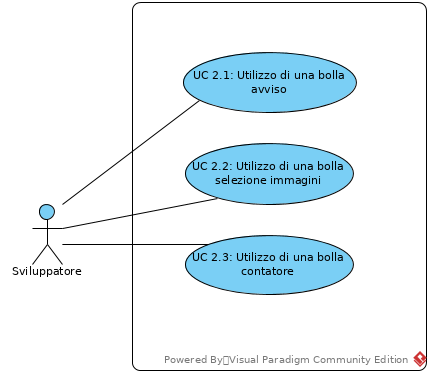
\includegraphics[scale=0.60]{Usecases/img/UC2.png}
	\caption{Caso d'uso UC 2: Utilizzo di bolle predefinite dell'SDK.}
\end{figure}

\FloatBarrier
\begin{itemize}
\item \textbf{Attori:} Sviluppatore.
\item \textbf{Descrizione:} Lo sviluppatore vuole utilizzare una bolla predefinita presente nell'SDK ovvero una tra le seguenti:
\begin{itemize}
\item Bolla avviso.
\item Bolla testo markdown.
\item Bolla lista.
\end{itemize} 
\item \textbf{Precondizione:} Lo sviluppatore vuole utilizzare una bolla predefinita presente nell'SDK. 
\item \textbf{Postcondizione:} Lo sviluppatore ha utilizzato una delle bolle predefinite presenti nella libreria di \progetto.
\item \textbf{Scenario principale:}
	\begin{itemize}
	\item{Utilizzo di una bolla avviso (UC 2.1).}
	\item{Utilizzo di una bolla testo markdown (UC 2.2).}
	\item{Utilizzo di una bolla lista (UC 2.3).}
	\end{itemize}
\end{itemize}
\subsubsection{Caso d'uso UC 2.1: Aggiunta di un metodo ad una bolla}

\FloatBarrier
\begin{itemize}
\item\textbf{Attori}: Sviluppatore.
\item\textbf{Descrizione}: Lo sviluppatore vuole aggiungere un nuovo metodo ad una bolla predefinita.
\item\textbf{Precondizione}: Lo sviluppatore vuole modificare il comportamento di una bolla predefinita presente in \progetto.
\item\textbf{Postcondizione}: Lo sviluppatore ha generato codice eseguibile per creare una nuova bolla derivata aggiungendo un metodo ad una bolla predefinita.
\end{itemize}
\subsubsection{Caso d'uso UC 2.2: Utilizzo di una bolla testo markdown}

\FloatBarrier
\begin{itemize}
\item\textbf{Attori}: Sviluppatore.
\item\textbf{Descrizione}: Lo sviluppatore vuole utilizzare una bolla predefinita di testo markdown. Questa bolla viene creata tramite l'inserimento di testo, scritto tramite la procedura di markdown.
\item\textbf{Precondizione}: Lo sviluppatore vuole utilizzare una bolla predefinita presente in \progetto.
\item\textbf{Postcondizione}: Lo sviluppatore ha generato codice eseguibile per creare una nuova bolla testo markdown.
\item\textbf{Scenario Principale}: Lo sviluppatore crea una bolla predefinita presente in \progetto.
\end{itemize}
\subsubsection{Caso d'uso UC 2.3: Utilizzo di una bolla lista}

\FloatBarrier
\begin{itemize}
\item\textbf{Attori}: Sviluppatore.
\item\textbf{Descrizione}: Lo sviluppatore vuole utilizzare la bolla lista predefinita. Questa bolla viene rappresenta la lista di elementi selezionabili.
\item\textbf{Precondizione}: Lo sviluppatore vuole utilizzare una bolla predefinita presente in \progetto.
\item\textbf{Postcondizione}: Lo sviluppatore ha generato codice eseguibile per creare una nuova bolla lista.
\item\textbf{Scenario Principale}: Lo sviluppatore crea una bolla predefinita presente in \progetto.
\end{itemize}
\subsection{Caso d'uso UC 3: Creazione di un widget personalizzato.}
\label{Caso d'uso UC 3: Creazione di un widget personalizzato.}

\FloatBarrier
\begin{itemize}
\item \textbf{Attori:} Sviluppatore.
\item \textbf{Descrizione:} Lo sviluppatore vuole creare un nuovo widget personalizzato.
\item \textbf{Precondizione:} Lo sviluppatore vuole creare un nuovo widget personalizzato. 
\item \textbf{Postcondizione:} Lo sviluppatore ha creato un nuovo widget personalizzato.
\item \textbf{Scenario principale:}
	\begin{itemize}
	\item{Lo sviluppatore vuole creare un nuovo widget personalizzato.}
	\end{itemize}
\end{itemize}
\newpage
\subsection{Caso d'uso UC 4: Applicazione demo lista-spesa.}
\label{Caso d'uso UC 4: Applicazione demo lista-spesa.}
\begin{figure}[ht]
	\centering
	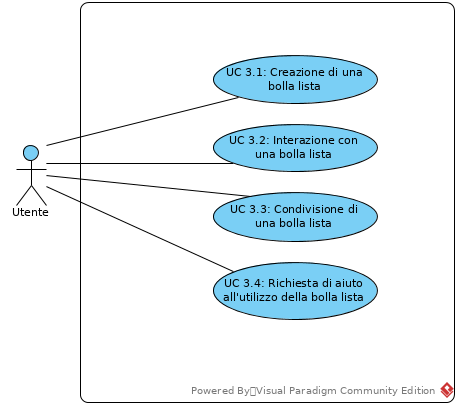
\includegraphics[scale=0.60]{Usecases/img/UC4.png}
	\caption{Caso d'uso UC 4: Applicazione demo lista spesa.}
\end{figure}



\FloatBarrier
\begin{itemize}
\item \textbf{Attori:} Utente.
\item \textbf{Descrizione:} L'utente utilizza l'applicazione demo lista-spesa.
\item \textbf{Precondizione:} L'utente vuole utilizzare l'applicazione demo lista-spesa. 
\item \textbf{Postcondizione:} L'utente ha utilizzato l'applicazione demo lista-spesa.
\item \textbf{Scenario principale:}
	\begin{itemize}
	\item{Creazione di una bolla lista-spesa (UC 4.1).}
	\item{Interazione con una bolla lista-spesa (UC 4.2).}
	\item{Condivisione di una bolla lista-spesa (UC 4.3).}
	\item{Richiesta di aiuto all'utilizzo della bolla lista spesa (UC 4.4).}
	\end{itemize}


\end{itemize}
\subsubsection{Caso d'uso UC 4.1: Configurazione di una bolla lista-spesa}
\label{Caso d'uso UC 4.1: Configurazione di una bolla lista-spesa}
\begin{figure}[ht]
	\centering
	\includegraphics[scale=0.80]{Usecases/img/{UC4.1}.png}
	\caption{Caso d'uso UC 4.1: Configurazione di una bolla lista-spesa}
\end{figure}
\FloatBarrier
\begin{itemize}
\item\textbf{Attori}: Creatore della lista.
\item\textbf{Descrizione}: L'attore crea la bolla lista-spesa e la configura.
\item\textbf{Precondizione}: L'attore vuole creare una bolla lista-spesa.
\item\textbf{Postcondizione}: Lo sviluppatore ha creato una bolla lista-spesa configurata.
\item\textbf{Estensioni}:
\begin{itemize}
		\item Impostazione del nome della lista a default(UC 4.1.2).
	\end{itemize}
	
\item\textbf{Scenario principale}:
	\begin{itemize}
		\item L'attore imposta il nome della lista-spesa(UC 4.1.1).
		\item L'attore imposta l'immagine della lista-spesa(UC 4.1.3).
	\end{itemize}
\item\textbf{Scenario alternativo}:
	\begin{itemize}
		\item L'attore non imposta il nome della lista oppure non lo imposta in modo non corretto(UC 4.1.2).
	\end{itemize}

\end{itemize}

\paragraph{Caso d'uso UC 4.1.1 Impostazione del nome della lista.}
	\begin{itemize}
	\item\textbf{Attori}: Creatore della lista.
		\item\textbf{Descrizione}: L'attore imposta il nome della lista.
		\item\textbf{Precondizione}: L'attore sta creando una bolla lista-spesa.
		\item\textbf{Postcondizione}: La bolla viene configurata con un nome desiderato.
		\item\textbf{Estensioni}: Impostazione del nome della lista a default(UC 4.1.2).
		\item\textbf{Scenario principale:} L'attore che sta creando la lista imposta il nome desiderato(UC 4.1.1).
		\item\textbf{Scenario alternativo:} L'attore che sta creando la lista non imposta il nome(UC 4.1.2)
		
	\end{itemize}

\paragraph{Caso d'uso UC 4.1.2 Impostazione del nome della lista a default.}
	\begin{itemize}
	\item\textbf{Attori}: Creatore della lista.
		\item\textbf{Descrizione}: La bolla viene impostata con un nome di default.
		\item\textbf{Precondizione}: L'attore non imposta il nome della lista oppure non lo imposta in modo non corretto.
		\item\textbf{Postcondizione}: La bolla viene configurata con un nome di default.
		\item\textbf{Scenario principale}: Il nome della lista, a causa di un mancato inserimento, viene impostato a default(UC 4.1.2).
		
	\end{itemize}
	
	
\paragraph{Caso d'uso UC 4.1.3 Impostazione dell'immagine della lista.}
	\begin{itemize}
	\item\textbf{Attori}: Creatore della lista.
		\item\textbf{Descrizione}: L'attore imposta l'immagine della lista.
		\item\textbf{Precondizione}: L'attore sta creando una bolla lista-spesa.
		\item\textbf{Postcondizione}: La bolla viene configurata con l'immagine desiderata.
		
		\item\textbf{Scenario principale:} L'attore che sta creando la lista imposta l'immagine desiderata(UC 4.1.3).
		
		
	\end{itemize}
	
\newpage
\subsubsection{Caso d'uso UC 4.2: Interazione con la bolla lista-spesa.}
\label{Caso d'uso UC 4.2: Interazione con la bolla lista-spesa.}
\begin{figure}[ht]
	\centering
	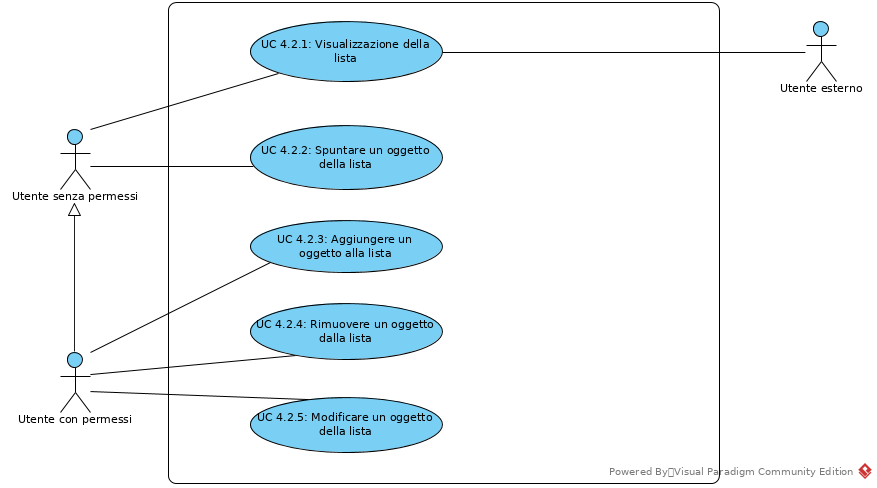
\includegraphics[scale=0.60]{Usecases/img/UC4.2.png}
	\caption{Caso d'uso UC 4.2: Interazione con la bolla lista-spesa.}
\end{figure}

\FloatBarrier
\begin{itemize}
\item \textbf{Attori:} Utente senza permessi, Utente con permessi, Utente esterno.
\item \textbf{Descrizione:} L'utente vuole interagire con la bolla lista-spesa e in base al tipo di utente potrà eseguire diverse azioni tra cui:
\begin{itemize}
\item Visualizzare la lista.
\item Spuntare un oggetto della lista.
\item Aggiungere un oggetto alla lista.
\item Rimuovere un oggetto dalla lista.
\item Modificare un oggetto della lista.
\end{itemize}
\item \textbf{Precondizione:} L'utente vuole interagire con la bolla lista-spesa. 
\item \textbf{Postcondizione:} L'utente ha interagito con la bolla lista-spesa con le modalità che la tipologia d'utente di cui fa parte permette.
\item \textbf{Scenario principale:}
	\begin{itemize}
	\item{Visualizzazione della lista (UC 4.2.1).}
	\item{Spunta di un oggetto della lista (UC 4.2.2).}
	\item{Aggiunta di un oggetto alla lista (UC 4.2.3).}
	\item{Rimozione di un oggetto dalla lista (UC 4.2.4).}
	\item{Richiesta di aiuto all'utilizzo della bolla lista spesa (UC 4.2.5).}
	\end{itemize}
\end{itemize}
\paragraph{Caso d'uso UC 4.2.1: Visualizzazione della lista.}
\label{Caso d'uso UC 4.2.1: Visualizzazione della lista.}

\FloatBarrier
\begin{itemize}
\item \textbf{Attori:} Utente senza permessi, Utente con permessi, Utente esterno.
\item \textbf{Descrizione:} L'utente vuole visualizzare la bolla lista-spesa.
\item \textbf{Precondizione:} L'utente vuole visualizzare la bolla lista-spesa. 
\item \textbf{Postcondizione:} L'utente ha visualizzato la bolla lista-spesa.
\item \textbf{Scenario principale:}
	\begin{itemize}
	\item{L'utente visualizza la bolla lista-spesa.}
	\end{itemize}
\end{itemize}
\subsection{Caso d'uso UC 4.2.2: Spunta di un oggetto della lista.}
\label{Caso d'uso UC 4.2.2: Spunta di un oggetto della lista.}

\FloatBarrier
\begin{itemize}
\item \textbf{Attori:} Utente senza permessi, Utente con permessi.
\item \textbf{Descrizione:} L'utente vuole spuntare un oggetto della bolla lista-spesa.
\item \textbf{Precondizione:} L'utente vuole spuntare un oggetto della bolla lista-spesa. 
\item \textbf{Postcondizione:} L'utente ha spuntato un oggetto della bolla lista-spesa.
\item \textbf{Scenario principale:}
	\begin{itemize}
	\item{L'utente spunta un oggetto della bolla lista-spesa.}
	\end{itemize}
\end{itemize}
\subsection{Caso d'uso UC 4.2.3: Aggiunta di un oggetto alla lista.}
\label{Caso d'uso UC 4.2.3: Aggiunta di un oggetto alla lista.}

\FloatBarrier
\begin{itemize}
\item \textbf{Attori:} Utente con permessi.
\item \textbf{Descrizione:} L'utente vuole aggiungere un oggetto alla bolla lista-spesa.
\item \textbf{Precondizione:} L'utente vuole aggiungere un oggetto alla bolla lista-spesa. 
\item \textbf{Postcondizione:} L'utente ha aggiunto un oggetto alla bolla lista-spesa.
\item \textbf{Scenario principale:}
	\begin{itemize}
	\item{L'utente aggiunge un oggetto alla bolla lista-spesa.}
	\end{itemize}
\end{itemize}
\paragraph{Caso d'uso UC 4.2.4: Rimozione di un prodotto dalla lista.}
\label{Caso d'uso UC 4.2.4: Rimozione di un prodotto dalla lista.}

\FloatBarrier
\begin{itemize}
\item \textbf{Attori:} Utente con permessi.
\item \textbf{Descrizione:} L'utente vuole rimuovere un oggetto dalla bolla lista-spesa.
\item \textbf{Precondizione:} L'utente vuole rimuovere un oggetto dalla bolla lista-spesa. 
\item \textbf{Postcondizione:} L'utente ha rimosso un oggetto dalla bolla lista-spesa.
\item \textbf{Scenario principale:}
	\begin{itemize}
	\item{L'utente rimuove un oggetto dalla bolla lista-spesa.}
	\end{itemize}
\end{itemize}
\paragraph{Caso d'uso UC 4.2.5: Modificare un oggetto della lista}
\label {Caso d'uso UC 4.2.5: Modificare un oggetto della lista}
\begin{figure}[ht]
	\centering
	\includegraphics[scale=0.80]{Usecases/img/{UC4.2.5}.png}
	\caption {Caso d'uso UC 4.2.5: Modificare un oggetto della lista}
\end{figure}
\FloatBarrier
\begin{itemize}
\item\textbf{Attori}: Utente con permessi.
\item\textbf{Descrizione}: L'attore modifica un oggetto della lista
\item\textbf{Precondizione}: L'attore ha i permessi per la modifica di un oggetto della lista.
\item\textbf{Postcondizione}: L'oggetto della lista viene modificato.
\item\textbf{Estensioni}:
	\begin{itemize}
		\item Visualizzazione messaggio d'errore(UC 4.2.5.2).
		\item Impostazione della quantità di prodotto richiesta a default(UC 4.2.5.7).
		\item Impostazione dell'unità di misura della quantità richiesta a default(UC 4.2.5.9). 
	\end{itemize}

	
\item\textbf{Scenario principale}:
	\begin{itemize}
		\item Modifica del nome del prodotto(UC 4.2.5.1).
		\item Modifica dell'immagine del prodotto(UC 4.2.5.3).
		\item Modifica della descrizione del prodotto(UC 4.2.5.4).
		\item Modifica delle note relative al prodotto(UC 4.2.5.5).
		\item Modifica della quantità richiesta di prodotto(UC 4.2.5.6).
		\item Modifica dell'unità di misura relativa alla quantità richiesta di prodotto(UC 4.2.5.8).
	\end{itemize}
\item\textbf{Scenario alternativo}:
	\begin{itemize}
		\item L'attore visualizza un messaggio d'errore a causa del mancato inserimento del nome del prodotto(UC 4.2.5.2).
		\item La quantità di prodotto viene aggiornata a default a causa del mancato inserimento di essa(UC 4.2.5.7).
		\item L'unità di misura della quantità di prodotto viene aggiornata a default a causa del mancato inserimento di essa(UC 4.2.5.9).
	\end{itemize}

\end{itemize}


\subparagraph{Caso d'uso UC 4.2.5.2 Visualizzazione messaggio d'errore.}
	\begin{itemize}
		\item\textbf{Attori}: Creatore della lista.
		\item\textbf{Descrizione}: L' attore visualizza un messaggio d'errore a causa del mancato inserimento del nome del prodotto.
		\item\textbf{Precondizione}: L' attore non imposta il nome del prodotto che vuole modificare.
		\item\textbf{Postcondizione}: L' attore visualizza un messaggio d'errore.
		\item\textbf{Scenario principale}:
			\begin{itemize}
				\item L'attore visualizza un messaggio d'errore. 
			\end{itemize}
		
	\end{itemize}
	
\subparagraph{Caso d'uso UC 4.2.5.7 Impostazione della quantità di prodotto richiesta a default.}
	\begin{itemize}
		\item\textbf{Attori}: Creatore della lista.
		\item\textbf{Descrizione}: La quantità di prodotto richiesta viene impostata a default a causa del mancato inserimento di essa.
		\item\textbf{Precondizione}: L'attore non imposta la quantità di prodotto che vuole modificare.
		\item\textbf{Postcondizione}:Il prodotto modificato ha una quantità  impostata a default.
		\item\textbf{Scenario principale}:
			\begin{itemize}
				\item La quantità del prodotto viene impostata a default.
			\end{itemize}
		
	\end{itemize}
\subparagraph{Caso d'uso UC 4.2.5.9 Impostazione dell'unità di misura della quantità richiesta a default.}
	\begin{itemize}
		\item\textbf{Attori}: Creatore della lista.
		\item\textbf{Descrizione}: L'unità di misura della quantità di prodotto richiesta viene impostata a default a causa del mancato inserimento di essa.
		\item\textbf{Precondizione}: L'attore non imposta l'unità di misura della quantità di prodotto che vuole modificare.
		\item\textbf{Postcondizione}: Il prodotto ha un unità di misura impostata a default.
		\item\textbf{Scenario principale}:
			\begin{itemize}
				\item L'unità di misura della quantità del prodotto viene impostata a default.
			\end{itemize}
		
\end{itemize}

\subsection{Caso d'uso UC 4.3: Condivisione di una bolla lista-spesa.}
\label{Caso d'uso UC 4.3: Condivisione di una bolla lista-spesa.}
\begin{figure}[ht]
	\centering
	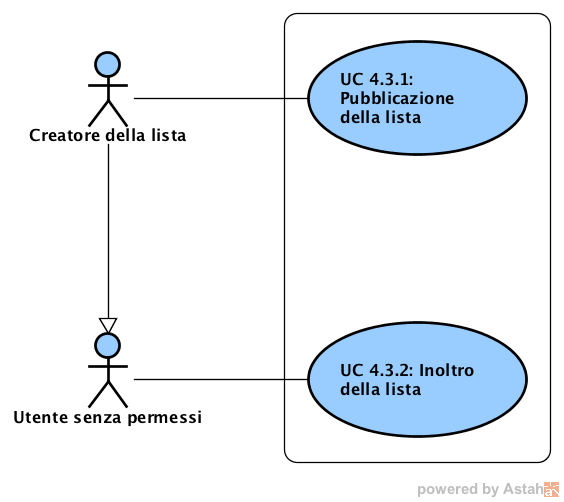
\includegraphics[scale=0.60]{Usecases/img/UC4.3.png}
	\caption{Caso d'uso UC 4.3: Condivisione di una bolla lista-spesa.}
\end{figure}

\FloatBarrier
\begin{itemize}
\item \textbf{Attori:} Utente.
\item \textbf{Descrizione:} L'utente utilizza l'applicazione demo lista-spesa.
\item \textbf{Precondizione:} L'utente vuole utilizzare l'applicazione demo lista-spesa. 
\item \textbf{Postcondizione:} L'utente ha utilizzato l'applicazione demo lista-spesa.
\item \textbf{Scenario principale:}
	\begin{itemize}
	\item{Creazione di una bolla lista-spesa (UC 4.1).}
	\item{Interazione con una bolla lista-spesa (UC 4.2).}
	\item{Condivisione di una bolla lista-spesa (UC 4.3).}
	\item{Richiesta di aiuto all'utilizzo della bolla lista spesa (UC 4.4).}
	\end{itemize}
\end{itemize}
\paragraph{Caso d'uso UC 4.3.1: Pubblicazione della lista.}
\label{Caso d'uso UC 4.3.1: Pubblicazione della lista.}

\FloatBarrier
\begin{itemize}
\item \textbf{Attori:} Creatore della lista.
\item \textbf{Descrizione:} Il Creatore della lista vuole pubblicare la bolla lista-spesa creata e può farlo in due modi:
\begin{itemize}
\item Pubblicando la bolla lista-spesa a un gruppo.
\item Pubblicando la bolla lista-spesa ad un utente.
\end{itemize}
\item \textbf{Precondizione:} Il Creatore della lista vuole pubblicare la bolla lista-spesa creata. 
\item \textbf{Postcondizione:} Il Creatore della lista ha pubblicato la bolla lista-spesa creata.
\item \textbf{Scenario principale:}
	\begin{itemize}
	\item{Pubblicazione della lista a un gruppo (UC 4.3.1.1).}
	\item{Pubblicazione della lista ad un utente (UC 4.3.1.4).}
	\end{itemize}
\end{itemize}
\subsection{Caso d'uso UC 4.3.1.1: Pubblicazione della lista a un gruppo.}
\label{Caso d'uso UC 4.3.1.1: Pubblicazione della lista a un gruppo.}

\FloatBarrier
\begin{itemize}
\item \textbf{Attori:} Creatore della lista.
\item \textbf{Descrizione:} Il Creatore della lista vuole pubblicare la bolla lista-spesa creata a un gruppo.
\item \textbf{Precondizione:} Il Creatore della lista vuole pubblicare la bolla lista-spesa creata a un gruppo. 
\item \textbf{Postcondizione:} Il Creatore della lista ha pubblicato a un gruppo la bolla lista-spesa creata.
\item \textbf{Inclusioni:}
	\begin{itemize}
	\item{Concessione ai partecipanti del gruppo dei permessi (UC 4.3.1.2).}
	\end{itemize}
\item \textbf{Scenario principale:}
	\begin{itemize}
	\item{Concessione ai partecipanti del gruppo dei permessi (UC 4.3.1.2).}
	\end{itemize}
\end{itemize}
\subparagraph{Caso d'uso UC 4.3.1.2: Concessione ai partecipanti del gruppo dei permessi.}
\label{Caso d'uso UC 4.3.1.2: Concessione ai partecipanti del gruppo dei permessi.}

\FloatBarrier
\begin{itemize}
\item \textbf{Attori:} Creatore della lista.
\item \textbf{Descrizione:} Il Creatore della lista vuole concedere ad alcuni partecipanti del gruppo i permessi di interazione con la bolla lista-spesa creata.
\item \textbf{Precondizione:} Il Creatore della lista vuole concedere ad alcuni partecipanti del gruppo i permessi di interazione con la bolla lista-spesa creata. 
\item \textbf{Postcondizione:} Il Creatore della lista ha concesso ad alcuni partecipanti del gruppo i permessi di interazione con la bolla lista-spesa creata.
\item \textbf{Estensioni:}
	\begin{itemize}
	\item{Permessi concessi a nessun partecipante (UC 4.3.1.3).}
	\end{itemize}
\item \textbf{Scenario principale:}
\begin{itemize}
\item Il Creatore della lista concede ad alcuni partecipanti del gruppo i permessi di interazione con la bolla lista-spesa creata.
\end{itemize}
\item \textbf{Scenario alternativo:}
	\begin{itemize}
	\item{Permessi concessi a nessun partecipante (UC 4.3.1.3).}
	\end{itemize}
\end{itemize}
\subsection{Caso d'uso UC 4.3.1.3: Permessi concessi a nessun partecipante.}
\label{Caso d'uso UC 4.3.1.3: Permessi concessi a nessun partecipante.}

\FloatBarrier
\begin{itemize}
\item \textbf{Attori:} Creatore della lista.
\item \textbf{Descrizione:} Il Creatore della lista non ha impostato per i partecipanti del gruppo i permessi di interazione con la bolla lista-spesa creata non concedendo di conseguenza i permessi di interazione con la bolla lista-spesa a nessun partecipante del gruppo.
\item \textbf{Precondizione:} Il Creatore della lista non ha impostato i permessi di interazione con la bolla lista-spesa creata per i partecipanti del gruppo.
\item \textbf{Postcondizione:} Il Creatore della lista non ha concesso a nessun partecipante del gruppo i permessi di interazione con la bolla lista-spesa.
\item \textbf{Scenario principale:}
\begin{itemize}
\item Il Creatore della lista non ha impostato per i partecipanti del gruppo i permessi di interazione con la bolla lista-spesa creata non concedendo di conseguenza i permessi di interazione con la bolla lista-spesa a nessun partecipante del gruppo.
\end{itemize}
\end{itemize}
\subsection{Caso d'uso UC 4.3.1.4: Pubblicazione della lista ad un utente.}
\label{Caso d'uso UC 4.3.1.4: Pubblicazione della lista ad un utente.}

\FloatBarrier
\begin{itemize}
\item \textbf{Attori:} Creatore della lista.
\item \textbf{Descrizione:} Il Creatore della lista vuole pubblicare la bolla lista-spesa creata ad un utente.
\item \textbf{Precondizione:} Il Creatore della lista vuole pubblicare la bolla lista-spesa creata ad un utente. 
\item \textbf{Postcondizione:} Il Creatore della lista ha pubblicato ad un utente la bolla lista-spesa creata.
\item \textbf{Inclusioni:}
	\begin{itemize}
	\item{Concessione all'utente dei permessi (UC 4.3.1.5).}
	\end{itemize}
	\item \textbf{Scenario principale:}
	\begin{itemize}
	\item{Concessione all'utente dei permessi (UC 4.3.1.5).}
	\end{itemize}
\end{itemize}
\subparagraph{Caso d'uso UC 4.3.1.5: Concessione all'utente dei permessi.}
\label{Caso d'uso UC 4.3.1.5: Concessione all'utente dei permessi.}

\FloatBarrier
\begin{itemize}
\item \textbf{Attori:} Creatore della lista.
\item \textbf{Descrizione:} Il Creatore della lista vuole concedere all'utente i permessi di interazione con la bolla lista-spesa creata.
\item \textbf{Precondizione:} Il Creatore della lista vuole concedere all'utente i permessi di interazione con la bolla lista-spesa creata. 
\item \textbf{Postcondizione:} Il Creatore della lista ha concesso all'utente i permessi di interazione con la bolla lista-spesa creata.
\item \textbf{Estensioni:}
	\begin{itemize}
	\item{Permessi non concessi all'utente (UC 4.3.1.6).}
	\end{itemize}
\item \textbf{Scenario principale:}
\begin{itemize}
\item Il Creatore della lista concede all'utente i permessi di interazione con la bolla lista-spesa creata.
\end{itemize}
\item \textbf{Scenario alternativo:}
\begin{itemize}
\item Permessi non concessi all'utente (UC 4.3.1.6).
\end{itemize}
\end{itemize}
\subparagraph{Caso d'uso UC 4.3.1.6: Permessi non concessi all'utente.}
\label{Caso d'uso UC 4.3.1.6: Permessi non concessi all'utente.}

\FloatBarrier
\begin{itemize}
\item \textbf{Attori:} Creatore della lista.
\item \textbf{Descrizione:} Il Creatore della lista non ha impostato per l'utente i permessi di interazione con la bolla lista-spesa creata non concedendo di conseguenza i permessi di interazione con la bolla lista-spesa all'utente.
\item \textbf{Precondizione:} Il Creatore della lista non ha impostato i permessi di interazione con la bolla lista-spesa creata per l'utente.
\item \textbf{Postcondizione:} Il Creatore della lista non ha concesso all'utente i permessi di interazione con la bolla lista-spesa.
\item \textbf{Scenario principale:}
\begin{itemize}
\item Il Creatore della lista non ha impostato per l'utente i permessi di interazione con la bolla lista-spesa non concedendo di conseguenza i permessi di interazione con la bolla lista-spesa all'utente.
\end{itemize}
\end{itemize}
\subsection{Caso d'uso UC 4.3.2: Inoltro della lista.}
\label{Caso d'uso UC 4.3.2: Inoltro della lista.}

\FloatBarrier
\begin{itemize}
\item \textbf{Attori:} Utente senza permessi.
\item \textbf{Descrizione:} L'utente vuole inoltrare in formato testuale la bolla lista-spesa per permetterne la sola visualizzazione.
\item \textbf{Precondizione:} L'utente vuole inoltrare in formato testuale la bolla lista-spesa. 
\item \textbf{Postcondizione:} L'utente ha inoltrato in formato testuale la bolla lista-spesa.
\item \textbf{Scenario principale:}
	\begin{itemize}
	\item L'utente inoltra in formato testuale la bolla lista-spesa per permetterne la sola visualizzazione.
	\end{itemize}
\end{itemize}
\newpage
\section{Requisiti}
Per poter svolgere al meglio le fasi di \PA\ e \PD\ dovrà essere stilato un elenco di requisiti emersi durante le riunioni interne e/o esterne. Tale compito spetta agli \textit{\AnP}. I requisiti dovranno
essere classificati secondo la seguente codifica:

\begin{center}
R-[Importanza][Tipo][Identificativo]
\end{center}
\begin{itemize}
	\item \textbf{Importanza:} può assumere questi valori:
  		\begin{itemize}
    		\item \textbf{1:} indica un requisito obbligatorio;
    		\item \textbf{2:} indica un requisito desiderabile;
    		\item \textbf{3:} indica un requisito facoltativo.
  		\end{itemize}
  	\item \textbf{Tipo:} può assumere questi valori:
  		\begin{itemize}
   		 	\item \textbf{F:} indica un requisito funzionale;
    		\item \textbf{Q:} indica un requisito di qualità;
    		\item \textbf{P:} indica un requisito prestazionale;
    		\item \textbf{V:} indica un requisito di vincolo.
  		\end{itemize}
  	\item \textbf{Identificativo:} indica il codice identificativo del requisito, è univoco e deve essere indicato in forma gerarchica.
\end{itemize}
Per ogni requisito si dovranno inoltre indicare:
\begin{itemize}
  \item \textbf{Descrizione:} una breve descrizione del requisito, che chiarisca tutti i punti di esso senza lasciare spazio a possibili ambiguità;
  \item \textbf{Fonte:} la fonte può essere una delle seguenti:
  \begin{itemize}
    \item \textit{\termine{Capitolato}}: deriva direttamente dal testo del capitolato;
    \item \textit{Verbale}: deriva da un incontro verbalizzato, seguito dall'identificativo dell'incontro;
    \item \textit{Interno}: deriva da discussioni interne al \termine{team};
    \item \textit{Caso d'uso}: deriva da uno o più casi d'uso e viene indicato tramite l'identificativo del caso o dei casi d'uso interessati.
  \end{itemize}
\end{itemize}

\newpage
\subsection{Requisiti Funzionali}
\normalsize
\begingroup
\renewcommand\arraystretch{2}
\begin{longtable}{|c|>{\centering}m{7cm}|c|}
\hline
\textbf{Id Requisito} & \textbf{Descrizione} & \textbf{Fonti}\\
\hline
\endhead
			R1F1 & Deve essere possibile creare alcune tipologie di bolle già definite all'interno dell'\termine{SDK} & Interno, UC1 \\
			\hline
			R1F1.1 & All'interno dell'\termine{SDK} deve essere possibile aggiungere un widget di tipo testo formattato e disporlo in qualsiasi modo all'interno della bolla & Interno, UC1.1, UC1, UC1.6 \\
			\hline
			R1F1.2 & All'interno dell'\termine{SDK} deve essere possibile aggiungere un widget di tipo immagine e disporlo in qualsiasi modo all'interno della bolla & Interno, UC1.2, UC1, UC1.6 \\ 
			\hline
			R1F1.3 & All'interno dell'\termine{SDK} deve essere possibile aggiungere un widget di tipo pulsante e disporlo in qualsiasi modo all'interno della bolla & Interno, UC1.3, UC1, UC1.6 \\ 
			\hline
			R1F1.4 & All'interno dell'\termine{SDK} deve essere possibile aggiungere un widget di tipo checklist e disporlo in qualsiasi modo all'interno della bolla & Interno, UC1.4, UC1, UC1.6 \\ 
			\hline
			R1F1.5 & All'interno dell'\termine{SDK} deve essere possibile aggiungere un widget personalizzato e disporlo in qualsiasi modo all'interno della bolla & Interno, UC1.5, UC1, UC1.6 \\ 
			\hline
			R2F1.1.1 & Deve essere possibile cambiare la dimensione del carattere con il quale è scritto il testo all'interno di un widget di testo formattato & Interno, UC1.1.1, UC1.1 \\
			\hline
			R1F1.1.2 & Se non viene inserita una grandezza del font personalizzata, oppure se ne viene inserita una non valida, deve essere impostata una grandezza di default & Interno, UC1.1.2, UC1.1\\
			\hline
			R2F1.1.3 & Deve essere possibile formattare parte del testo di un widget di testo formattato in corsivo & Interno, UC1.1.3, UC1.1 \\
			\hline
			R1F1.1.4 & Deve essere possibile inserire uno o più link cliccabili all'interno di un widget di tipo testo formattato & Interno, UC1.1.4, UC1.1 \\
			\hline
			R1F1.1.5 & Deve essere possibile impostare il colore del link cliccabile all'interno del widget di testo formattato & Interno, UC1.1.5, UC1.1 \\
			\hline
			R1F1.1.6 & Deve essere previsto un colore di default per i link cliccabili all'interno di un widget di testo formattato & Interno, UC1.1.6, UC1.1 \\
			\hline
			R2F1.1.7 & Deve essere possibile formattare parte del testo di un widget di testo formattato in grassetto & Interno, UC1.1.7, UC1.1 \\
			\hline
			R1F1.1.8 & Deve essere possibile impostare un colore personalizzato per parte del testo di un widget di testo formattato & Interno, UC1.1.8, UC1.1 \\
			\hline
			R1F1.1.9 & Deve essere previsto un colore di default per il testo di un widget di testo formattato & Interno, UC1.1.9, UC1.1 \\
			\hline
			R1F1.1.10 & Deve essere possibile aggiungere del testo ad un widget di tipo testo formattato & Interno, UC1.1.10, UC1.1 \\
			\hline
			R1F1.1.11 & Deve essere previsto un messaggio di errore dettagliato nell'evenienza in cui venga aggiunto del testo non valido ad un widget di tipo testo formattato.	& Interno, UC1.1.11, UC1.1 \\
			\hline
			R1F1.3.1 & Deve essere possibile aggiungere un widget che rappresenti un bottone semplice & Interno, UC1.3.1, UC1.3 \\
			\hline
			R1F1.3.2 & Deve essere possibile aggiungere un widget che rappresenti un check button & Interno, UC1.3.2, UC1.3 \\
			\hline
			R1F1.3.3 & Deve essere possibile impostare una azione personalizzata per ogni evento di un bottone & Interno, UC1.3.3, UC1.3 \\
			\hline
			R1F1.3.1.1 & Deve essere possibile impostare il testo presente all'interno di un bottone semplice & Interno, UC1.3.1.1, UC1.3.1 \\
			\hline
			R1F1.3.1.2 & Se viene inserito un testo non valido oppure vuoto come testo interno ad un bottone semplice, deve essere visualizzato un messaggio di errore & Interno, UC1.3.1.2, UC1.3.1 \\
			\hline
			R2F1.3.1.3 & Deve essere possibile impostare le dimensioni di un bottone presente all'interno di un widget & Interno, UC1.2.1.3, UC1.2.1 \\
			\hline
			R1F1.3.1.4 & Le dimensioni del bottone devono essere impostate a valori di default nel qual caso lo sviluppatore inserisca delle dimensioni personalizzate non valide & Interno, UC1.3.1.4, UC1.3.1 \\
			\hline
			R3F1.3.1.5 & Deve essere possibile impostare il colore di sfondo di un bottone & Interno, UC1.3.1.5, UC1.3.1 \\
			\hline
			R1F1.3.1.6 & Deve essere previsto un colore di sfondo di default nel qual caso lo sviluppatore non lo personalizzi oppure tenti di utilizzarne uno non valido & Interno, UC1.3.1.6, UC1.3.1 \\
			\hline
			R1F1.3.2.1 & Deve essere possibile impostare lo stato iniziale di un check button & Interno, UC1.3.2.1, UC1.3.2 \\
		\hline
		R1F1.3.2.2 & Deve essere previsto uno stato di default per i bottoni di check nel qual caso il loro stato non venga impostato ad un valore personalizzato & Interno, UC1.3.2.2, UC1.3.2 \\
		\hline
		R1F1.3.2.3 & Deve essere possibile personalizzare l'aspetto del bottone di check una volta che viene selezionato & Interno, UC1.3.2.3, UC1.3.2 \\
		\hline
		R2F1.3.2.3.1 & Deve essere possibile impostare la visualizzazione della selezione di un bottone di check mediante una "X" & Interno, UC1.3.2.3.1, UC1.3.2.3 \\ 
		\hline
		R1F1.3.2.3.2 & Deve essere possibile impostare la visualizzazione della selezione di un bottone di check mediante una spunta & Interno, UC1.3.2.3.2, UC1.3.2.3 \\ 
		\hline
		R2F1.3.2.3.3 & Deve essere possibile impostare la visualizzazione della selezione di un bottone di check mediante la colorazione stessa del bottone & Interno, UC1.2.2.3.3, UC1.3.2.3 \\ 
		\hline
		R3F1.3.2.3.4 & Deve essere possibile scegliere un colore personalizzato da utilizzare per indicare la selezione di un bottone di check & Interno, UC1.3.2.3.4, UC1.3.2.3 \\ 
		\hline
		R2F1.3.2.3.5 & Se non viene personalizzato, il colore di default utilizzato per l'indicazione della selezione di un bottone di check deve essere il verde & Interno, UC1.3.2.3.5, UC1.3.2.3 \\
		\hline
		R1F1.3.3.1 & Deve essere possibile impostare una azione da eseguire in seguito al click normale di un bottone & Interno, UC1.3.3.1, UC1.3.3\\ 
		\hline
		R2F1.3.3.2 & Deve essere possibile impostare una azione da eseguire in seguito al click prolungato di un bottone & Interno, UC1.3.3.2, UC1.3.3\\ 
		\hline
		R1F1.3.3.3 & Deve essere possibile impostare il tempo che deve intercorrere tra l'inizio della pressione e l'avvio dell'azione conseguente al click prolungato di un bottone & Interno, UC1.3.3.3, UC1.3.3\\ 
		\hline
		R3F1.3.3.4 & Deve essere previsto un valore di default per il tempo che deve intercorrere tra l'inizio del click prolungato di un bottone e l'avvio dell'azione associata & Interno, UC1.3.3.4, UC1.3.3\\ 
		\hline
		R1F1.4.1 & Deve essere possibile personalizzare l'elenco puntato di un widget di tipo checklist & Interno, UC1.4.1, UC1.4 \\
		\hline
		R1F1.4.2 & Deve essere possibile impostare un messaggio di completamento da visualizzare una volta che tutti gli elementi di una checklist sono stati segnati come selezionati & Interno, UC1.4.2, UC1.4 \\
		\hline
		R1F1.4.3 & Deve essere previsto un messaggio di errore da visualizzare nel qual caso si cerchi di impostare un messaggio di completamento non valido per un widget di checklist & Interno, UC1.4.3, UC1.4 \\
		\hline	
		R3F1.4.1.1 & Deve essere possibile visualizzare la lista di un widget di tipo checklist sotto forma di elenco numerato & Interno, UC1.4.1.1, UC1.4.1 \\
		\hline
		R1F1.4.1.2 & Deve essere possibile visualizzare la lista di un widget di tipo checklist sotto forma di elenco non numerato con indicatore un pallino & Interno, UC1.4.1.2, UC1.4.1 \\
		\hline
		R2F1.4.1.3 & Deve essere possibile visualizzare la lista di un widget di tipo checklist sotto forma di elenco non numerato con indicatore un trattino & Interno, UC1.4.1.3, UC1.4.1 \\
		\hline
		R1F1.2.1 & Deve essere possibile associare una immagine ad un widget di tipo immagine & Interno, UC1.2.1, UC1.2 \\
		\hline
		R1F1.2.2 & Deve essere previsto un messaggio di errore da visualizzare nel qual caso lo sviluppatore non associ una immagine ad un widget immagine oppure tenti di associarne una non supportata & Interno, UC1.2.2, UC1.2 \\
		\hline
		R2F1.2.3 & Deve essere possibile impostare delle dimensioni personalizzate all'immagine presente all'interno di un widget di tipo immagine & Interno, UC1.2.3, UC1.2 \\
		\hline
		R1F1.2.4 & Devono essere previste delle dimensioni di default nel qual caso lo sviluppatore tenti di personalizzare le dimensioni di una immagine all'interno di un widget immagine usando valori non validi & Interno,UC1.2.4, UC1.2 \\
			\hline
		R1F1.5.1 & Deve essere possibile modificare il testo già contenuto all'interno di un widget testo & Interno, UC1.1.10 \\
		\hline
		R1F1.5.2 & Deve essere possibile modificare l'immagine associata ad un widget di tipo immagine & Interno, UC1.2.1 \\
		\hline
		R1F1.5.3 & Deve essere previsto un messaggio d'errore nel qual caso lo sviluppatore tenti di modificare una immagine già esistente utilizzandone una non valida & Interno, UC1.2.2 \\
		\hline
		R1F1.5.1.1 & Deve essere possibile modificare parte del testo precedentemente formattato in corsivo all'interno di un widget di testo formattato & Interno, UC1.1.3 \\
		\hline
		R1F1.5.1.2 & Deve essere possibile modificare parte del testo precedentemente formattato in grassetto all'interno di un widget di testo formattato & Interno, UC1.1.7 \\
		\hline
		R1F1.5.1.3 & Deve essere possibile modificare la grandezza del carattere di parte del testo presente all'interno di un widget di testo formattato precedentemente creata & Interno, UC1.1.1\\
		\hline
		R1F1.5.1.4 & Deve essere prevista una grandezza del font di default da utilizzare nel qual caso la modifica della grandezza del font di un widget precedentemente venga utilizzata in modo scorretto & Interno, UC1.1.2 \\
		\hline
		R1F1.5.1.5 & Deve essere possibile modificare i link cliccabili precedentemente inseriti all'interno di un widget di testo formattato & Interno, UC1.1.4 \\
		\hline
		R2F1.5.1.6 & Deve essere possibile cambiare il colore dei link cliccabili presenti all'interno di un widget di testo formattato precedentemente creata & Interno, UC1.1.5 \\
		\hline
		R1F1.5.1.7 & Nel qual caso si tenti di modificare il colore dei link cliccabili presenti all'interno di un widget di testo formattato utilizzando un colore non valido, il colore di tali link deve essere impostato a blu & Interno, UC1.1.6 \\
		\hline
		R1F1.5.1.8 & Deve essere possibile modificare il colore precedentemente utilizzato per colorare parte del testo di un widget di tipo testo formattato & Interno, UC1.1.8 \\
		\hline
		R1F1.5.1.9 & Deve essere previsto un colore di default nel qual caso si tenti di modificare il colore di parte del testo di un widget di testo formattato utilizzando un valore non valido & Interno, UC1.1.9 \\
		\hline
		R1F1.5.1.10 & Deve essere possibile cambiare il testo presente all'interno di un widget precedentemente creata & Interno, UC1.1.10 \\
		\hline
		R1F1.5.1.11 & Deve essere previsto un messaggio di errore nel qual caso il testo che si vuole inserire in un widget non sia valido & Interno, UC1.1.11 \\
		\hline
			R1F2 & Deve essere possibile creare delle nuove bolle a partire da quelle già esistenti all'interno dell'\termine{SDK} & Interno, UC2 \\
			\hline
			R1F3 & Deve essere possibile accedere all'\termine{SDK} & Capitolato \\
			\hline
			R1F4 & Deve essere possibile creare facilmente delle bolle nuove & Capitolato \\
			\hline				
\caption[Requisiti Funzionali]{Requisiti Funzionali}
\label{tabella: Requisiti Funzionali}
\end{longtable}
\endgroup
\clearpage
\newpage
\subsection{Requisiti Qualità}
\normalsize
\begingroup
\renewcommand\arraystretch{2}
\begin{longtable}{|c|>{\centering}m{7cm}|c|}
\hline
\textbf{Id Requisito} & \textbf{Descrizione} & \textbf{Fonti}\\
\hline
\endhead
			R1Q1 & Deve essere fornito un manuale utente & \termine{Capitolato} \\
			\hline
			R1Q2 & Il manuale utente deve essere fornito in lingua inglese & \termine{Capitolato} \\
			\hline
			R1Q3 & La documentazione utile per l'utilizzatore finale, non contenuta nel manuale utente, dovrà essere scritta in inglese e allegata al manuale  & \termine{Capitolato} \\ 
			\hline
			R1Q4 & La documentazione formale e standard (i documenti che bisogna consegnare ad ogni revisione di progetto) deve essere scritta in italiano  & Interno, Verbale di riunione del 23/12/2016\\ 
			\hline
			R1Q5 & Il manuale utente deve contenere una parte dove vengono specificati e spiegati  i vari errori che si possono incontrare quando si usa l'\termine{SDK} sviluppato & Interno \\ 
			\hline
			R2Q6 & Il manuale utente deve spiegare in maniera semplice e concisa come installare \progettoShort\ in un server contenete \termine{Rocket.chat} & Interno \\ 
			\hline
			R1Q6 & L'applicazione sviluppata come demo deve essere documentata & \termine{Capitolato} \\ 
			\hline
\caption[Requisiti di Qualità]{Requisiti di Qualità}
\label{tabella: Requisiti Funzionali}
\end{longtable}
\endgroup
\clearpage
\newpage
\subsection{Requisiti Vincolo}
\normalsize
\begingroup
\renewcommand\arraystretch{2}
\begin{longtable}{|c|>{\centering}m{7cm}|c|}
\hline
\textbf{Id Requisito} & \textbf{Descrizione} & \textbf{Fonti}\\
\hline
\endhead
			R1V1 & Deve essere creato un \termine{SDK} per permettere agli sviluppatori di creare nuove bolle & \termine{Capitolato} \\
			\hline
			R1V2 & Le bolle interattive create tramite \progettoShort\ devono funzionare dentro una istanza del \termine{server} \termine{web chat} \termine{Rocket.chat} & \termine{Capitolato}   \\
			\hline
			R2V3 & Durante lo sviluppo deve essere disponibile un server sul quale vi è installata una istanza di \termine{Rocket.chat}  & Interno \\ 
			\hline
			R2V4 & Le bolle create devono ricadere in una delle seguenti tre tipologie:  \textit{Rich media bubble}, \textit{Self-updating bubble} o \textit{Editing bubble} & Capitolato\\ 
			\hline
			R1V5 & \progettoShort\ deve essere in grado di fornire bolle predefinite già pronte ad essere utilizzate da parte dell'utente finale  & \termine{Capitolato} \\ 
			\hline
			R1V6 & \progettoShort\ deve provvedere delle \termine{API} per permettere agli sviluppatori futuri di creare delle nuove bolle secondo i loro requisiti  & \termine{Capitolato} \\ 
			\hline
			R1V7 & Dovrà essere creata una demo significativa che mostri un interessante uso delle bolle all'interno di \termine{Rocket.chat} & \termine{Capitolato} \\ 
			\hline
			R1V8 & L'\termine{SDK} e la demo dovranno essere sviluppati in \termine{javascript} 6th edition usando il "\termine{promise centric approach}" ed evitando il più possibile le \termine{callback}
			 & \termine{Capitolato} \\ 
			\hline
			R1V9 & Le \termine{callback} qualora venissero usate devono essere giustificate in maniera corretta
			 & \termine{Capitolato} \\ 
			 \hline
			 R1V10 & Per scrivere la demo e l'\termine{SDK} bisogna seguire il più possibile le \termine{12 Factors app guidelines}
			 & \termine{Capitolato} \\ 
			\hline
			R2V11 & E' consigliato l'uso di un \termine{framework frontend}
			 & \termine{Capitolato} \\ 
			\hline
			R2V12 & E' consigliato l'uso di \termine{SCSS}
			 & \termine{Capitolato} \\ 
			\hline
			R1V12 & La demo dovrà essere usufruibile tramite \termine{Heroku} sotto forma di pacchetto indipendente
			 & \termine{Capitolato} \\ 
			\hline
			R1V13 & Il codice sorgente di \progettoShort\ dovrà essere caricato e versionato su \termine{GitHub} o  \termine{Bitbucket}
			 & \termine{Capitolato} \\ 
			\hline
			R1V14 & Utilizzo obbligatorio di \termine{linting} per mettere in evidenza utilizzi non corretti del linguaggio & Verbale\_2\_E\_2017-02-24 \\ 
			\hline
\caption[Requisiti di Vincolo]{Requisiti di Vincolo}
\label{tabella: Requisiti di Vincolo}
\end{longtable}
\endgroup
\clearpage
\subsection{Tracciamento Fonti-Requisiti}
\normalsize
\begin{longtable}{|>{\centering}m{5cm}|m{5cm}<{\centering}|}
\hline 
\textbf{Fonte} & \textbf{Id Requisiti}\\
\hline
\endhead
{Capitolato}&{R1F0}\\
&{R1Q2}\\
&{R1Q3}\\
&{R1Q6}\\
&{R1V1}\\
&{R2V3}\\
&{R1V4}\\
&{R1V5}\\
&{R1V6}\\
&{R1V7}\\
&{R1V8}\\
&{R2V9}\\
&{R2V10}\\
&{R1V11}\\
&{R1V12}\\ \hline
{Interno} & {R1F1}\\
&{R1F1.1}\\
&{R1F1.2}\\
&{R1F1.3}\\
&{R1F1.4}\\
&{R1F1.5}\\
&{R2F1.1.1}\\
&{R1F1.1.2}\\
&{R2F1.1.3}\\
&{R1F1.1.4}\\
&{R1F1.1.5}\\
&{R1F1.1.6}\\
&{R2F1.1.7}\\
&{R1F1.1.8}\\
&{R1F1.1.9}\\
&{R1F1.1.10}\\
&{R1F1.1.11}\\

&{R1F1.2.1}\\
&{R1F1.2.2}\\
&{R1F1.2.3}\\
&{R1F1.2.4}\\

&{R1F1.3.1}\\
&{R1F1.3.2}\\
&{R1F1.3.3}\\
&{R3F1.3.1.1}\\
&{R1F1.3.1.2}\\
&{R2F1.3.1.3}\\
&{R1F1.3.1.4}\\
&{R1F1.3.1.5}\\
&{R1F1.3.1.6}\\
&{R1F1.3.2.1}\\
&{R1F1.3.2.2}\\
&{R1F1.3.2.3}\\
&{R1F1.3.2.4}\\
&{R1F1.3.2.5}\\
&{R2F1.3.2.3.1}\\
&{R1F1.3.2.3.2}\\
&{R2F1.3.2.3.3}\\
&{R3F1.3.2.3.4}\\
&{R2F1.3.2.3.5}\\
&{R1F1.3.3.1}\\
&{R2F1.3.3.2}\\
&{R3F1.3.3.3}\\
&{R1F1.3.3.4}\\

&{R1F1.4.1}\\
&{R1F1.4.2}\\
&{R1F1.4.3}\\
&{R3F1.4.1.1}\\
&{R1F1.4.1.2}\\
&{R2F1.4.1.3}\\

&{R1F1.5.1}\\
&{R1F1.5.2}\\
&{R1F1.5.3}\\
&{R1F1.5.1.1}\\
&{R1F1.5.1.2}\\
&{R1F1.5.1.3}\\
&{R1F1.5.1.4}\\
&{R1F1.5.1.5}\\
&{R2F1.5.1.6}\\
&{R1F1.5.1.7}\\
&{R1F1.5.1.8}\\
&{R1F1.5.1.9}\\
&{R1F1.5.1.10}\\
&{R1F1.5.1.11}\\
&{R1F1.5.3.1}\\
&{R1F1.5.3.2}\\
&{R1F1.5.3.3}\\
&{R1F1.5.3.4}\\

&{R1F2}\\
&{R1F2.1}\\
&{R1F2.2}\\
&{R1F2.3}\\

&{R1F3}\\

&{R1Q4}\\
&{R1Q5}\\
&{R2Q6}\\ 

&{R2V2}\\
&{R1V13}\\

&{R1F4}\\
&{R1F4.1}\\
&{R1F4.1.1}\\
&{R1F4.1.2}\\
&{R1F4.1.3}\\
&{R1F4.1.4}\\
&{R1F4.1.5}\\
&{R1F4.2.1}\\
&{R1F4.2.2}\\
&{R1F4.2.3}\\
&{R3F4.2.4}\\
&{R1F4.2.5}\\
&{R1F4.2.3.1}\\
&{R1F4.2.3.2}\\
&{R1F4.2.3.3}\\
&{R1F4.2.3.4}\\
&{R1F4.2.3.5}\\
&{R1F4.2.3.6}\\
&{R1F4.2.3.7}\\
&{R1F4.2.3.8}\\
&{R1F4.2.3.9}\\
&{R3F4.2.4}\\
&{R1F4.2.5}\\
&{R1F4.2.5.1}\\
&{R1F4.2.5.2}\\
&{R1F4.2.5.3}\\
&{R1F4.2.5.4}\\
&{R1F4.2.5.5}\\
&{R1F4.2.5.6}\\
&{R1F4.2.5.7}\\
&{R1F4.2.5.8}\\
&{R1F4.2.5.9}\\
&{R1F4.3.1.1}\\
&{R1F4.3.1.2}\\
&{R1F4.3.1.3}\\
&{R1F4.3.1.4}\\
&{R1F4.3.1.5}\\
&{R1F4.3.1.6}\\
&{R1F4.3.1.7}\\
&{R1F4.3.2}\\
&{R1F4.3.3}\\ 
&{R1F4.3.4}\\ 
&{R1F4.3.5}\\ \hline

{Verbale 2016-12-23}&{R1Q4}\\ \hline
{Verbale\_2\_E\_2017-02-24}&{R1V13}\\ \hline
{UC1}&{R1F1}\\
&{R1F1.1}\\
&{R1F1.2}\\
&{R1F1.3}\\
&{R1F1.4}\\
&{R1F1.5}\\ \hline
{UC1.1}&{R1F1.1}\\
&{R2F1.1.1}\\
&{R1F1.1.2}\\
&{R2F1.1.3}\\
&{R1F1.1.4}\\
&{R1F1.1.5}\\
&{R1F1.1.6}\\
&{R2F1.1.7}\\
&{R1F1.1.8}\\
&{R1F1.1.9}\\
&{R1F1.1.10}\\
&{R1F1.1.11}\\ \hline
{UC1.2}&{R1F1.2}\\
&{R1F1.2.1}\\
&{R1F1.2.2}\\
&{R2F1.2.3}\\
&{R1F1.2.4}\\ \hline
{UC1.3}&{R1F1.3}\\
&{R1F1.3.1}\\
&{R1F1.3.2}\\
&{R1F1.3.3}\\
&{R1F1.3}\\ \hline
{UC1.4}&{R1F1.4}\\
&{R1F1.4.1}\\
&{R1F1.4.2}\\ 
&{R1F1.4.3}\\ \hline
{UC1.5}&{R1F1.5}\\ \hline
{UC1.6}&{R1F1.6}\\
&{R1F1.1}\\
&{R1F1.2}\\
&{R1F1.3}\\
&{R1F1.4}\\
&{R1F1.5}\\ \hline
{UC1.1.1}&{R2F1.1.1}\\
&{R1F1.5.1.3}\\ \hline
{UC1.1.2}&{R1F1.1.2}\\
&{R1F1.5.1.4}\\ \hline
{UC1.1.3}&{R2F1.1.3}\\
&{R1F1.5.1.1}\\ \hline
{UC1.1.4}&{R1F1.1.4}\\
&{R1F1.5.1.5}\\ \hline
{UC1.1.5}&{R1F1.1.5}\\
&{R2F1.5.1.6}\\ \hline
{UC1.1.6}&{R1F1.1.6}\\
&{R1F1.5.1.7}\\ \hline
{UC1.1.7}&{R2F1.1.7}\\
&{R1F1.5.1.2}\\ \hline
{UC1.1.8}&{R1F1.1.8}\\
&{R1F1.5.1.8}\\ \hline
{UC1.1.9}&{R1F1.1.9}\\
&{R1F1.5.1.9}\\ \hline
{UC1.1.10}&{R1F1.1.10}\\
&{R1F1.5.1}\\
&{R1F1.5.1.10}\\ \hline
{UC1.1.11}&{R1F1.1.11}\\
&{R1F1.5.1.11}\\ \hline

{UC1.2.1}&{R1F1.2.1}\\
&{R1F1.5.2.1}\\ \hline
{UC1.2.2}&{R1F1.2.2}\\
&{R1F1.5.2.2}\\ \hline
{UC1.2.3}&{R1F1.2.3}\\ \hline

{UC1.3.1}&{R1F1.3.1}\\
&{R1F1.3.1.1}\\
&{R1F1.3.1.2}\\
&{R2F1.3.1.3}\\
&{R1F1.3.1.4}\\
&{R3F1.3.1.5}\\
&{R1F1.3.1.6}\\ \hline
{UC1.3.2}&{R1F1.3.2}\\
&{R1F1.3.2.1}\\
&{R1F1.3.2.2}\\
&{R1F1.3.2.3}\\
&{R1F1.3.2.4}\\
&{R1F1.3.2.5}\\ \hline
{UC1.3.3}&{R1F1.3.3}\\
&{R1F1.3.3.1}\\
&{R2F1.3.2.2}\\
&{R1F1.3.2.3}\\
&{R3F1.3.2.4}\\ \hline
{UC1.3.1.1}&{R3F1.3.1.1}\\
&{R1F1.5.3.1}\\ \hline
{UC1.3.1.2}&{R1F1.3.1.2}\\
&{R1F1.5.3.3}\\ \hline
{UC1.3.1.3}&{R2F1.3.1.3}\\ \hline
{UC1.3.1.4}&{R1F1.3.1.4}\\ \hline
{UC1.3.1.5}&{R3F1.3.1.5}\\ \hline
{UC1.3.1.6}&{R1F1.3.1.6}\\ \hline
{UC1.3.2.1}&{R1F1.3.2.1}\\ \hline
{UC1.3.2.2}&{R1F1.3.2.2}\\ \hline
{UC1.3.2.3}&{R1F1.3.2.3}\\
&{R2F1.3.2.3.1}\\
&{R1F1.3.2.3.1}\\
&{R2F1.3.2.3.1}\\
&{R3F1.3.2.3.1}\\
&{R2F1.3.2.3.1}\\ \hline
{UC1.3.2.4}&{R1F1.3.2.4}\\
&{R1F1.5.3.2}\\ \hline
{UC1.3.2.5}&{R1F1.3.2.5}\\
&{R1F1.5.3.4}\\ \hline
{UC1.3.3.1}&{R1F1.3.3.1}\\ \hline
{UC1.3.3.2}&{R2F1.3.3.2}\\ \hline
{UC1.3.3.3}&{R1F1.3.3.3}\\ \hline
{UC1.3.3.4}&{R3F1.3.3.4}\\ \hline

{UC1.4.1}&{R1F1.4.1}\\
&{R3F1.4.1.1}\\
&{R1F1.4.1.2}\\
&{R1F1.4.1.3}\\ \hline
{UC1.4.2}&{R1F1.4.2}\\ \hline
{UC1.4.3}&{R2F1.4.3}\\ \hline
{UC1.4.1.1}&{R3F1.4.1.1}\\ \hline
{UC1.4.1.1}&{R3F1.4.1.2}\\ \hline
{UC1.4.1.1}&{R3F1.4.1.3}\\ \hline
{UC1.6}&{R1F1.6}\\ \hline
{UC1.7}&{R1F1.7}\\
&{R1F1.7.1}\\ \hline
{UC1.7.1}&{R1F1.7.1}\\
&{R1F1.7.1.1}\\
&{R1F1.7.1.2}\\
&{R1F1.7.1.3}\\
&{R1F1.7.1.4}\\
&{R1F1.7.1.5}\\ \hline
{UC1.7.1.1}&{R1F1.7.1.1}\\ \hline
{UC1.7.1.2}&{R1F1.7.1.2}\\ \hline
{UC1.7.1.3}&{R1F1.7.1.3}\\ \hline
{UC1.7.1.4}&{R1F1.7.1.4}\\ \hline
{UC1.7.1.5}&{R1F1.7.1.5}\\ \hline


{UC2}&{R1F2}\\
&{R1F2.1}\\
&{R1F2.2}\\
&{R1F2.3}\\ \hline
{UC2.1}&{R1F2.1}\\ \hline
{UC2.2}&{R1F2.2}\\ \hline
{UC2.3}&{R1F2.3}\\ \hline

{UC3}&{R1F3}\\ \hline

\caption[Tracciamento Fonti-Requisiti]{Tracciamento Fonti-Requisiti}
\label{tabella: Tracciamento Fonti-Requisiti}
\end{longtable}


\subsection{Tracciamento Fonti-Requisiti Demo}
\normalsize
\begin{longtable}{|>{\centering}m{5cm}|m{5cm}<{\centering}|}
\hline 
\textbf{Fonte} & \textbf{Id Requisiti}\\
\hline
\endhead

{UC4}&{R1F4}\\
&{R1F4.1}\\ \hline
{UC4.1}&{R1F4.1}\\
&{R1F4.1.1}\\
&{R1F4.1.2}\\
&{R1F4.1.3}\\
&{R1F4.1.4}\\
&{R1F4.1.5}\\
{UC4.1.1}&{R1F4.1.1}\\ \hline
{UC4.1.1}&{R1F4.1.2}\\ \hline
{UC4.1.1}&{R1F4.1.3}\\ \hline
{UC4.1.1}&{R1F4.1.4}\\ \hline
{UC4.1.1}&{R1F4.1.5}\\ \hline

{UC4.2}&{R1F4.2.1}\\
&{R1F4.2.2}\\
&{R1F4.2.3}\\
&{R3F4.2.4}\\
&{R1F4.2.5}\\
&{R1F4.2.3.1}\\
&{R1F4.2.3.2}\\
&{R1F4.2.3.3}\\
&{R1F4.2.3.4}\\
&{R1F4.2.3.5}\\
&{R1F4.2.3.6}\\
&{R1F4.2.3.7}\\
&{R1F4.2.3.8}\\
&{R1F4.2.3.9}\\ \hline
{UC4.2.1}&{R1F4.2.1}\\ \hline
{UC4.2.2}&{R1F4.2.2}\\ \hline
{UC4.2.3}&{R1F4.2.3}\\
&{R1F4.2.3.1}\\
&{R1F4.2.3.2}\\
&{R1F4.2.3.3}\\
&{R1F4.2.3.4}\\
&{R1F4.2.3.5}\\
&{R1F4.2.3.6}\\
&{R1F4.2.3.7}\\
&{R1F4.2.3.8}\\
&{R1F4.2.3.9}\\ \hline
{UC4.2.4}&{R3F4.2.4}\\ \hline
{UC4.2.5}&{R1F4.2.5}\\
&{R1F4.2.5.1}\\
&{R1F4.2.5.2}\\
&{R1F4.2.5.3}\\
&{R1F4.2.5.4}\\
&{R1F4.2.5.5}\\
&{R1F4.2.5.6}\\
&{R1F4.2.5.7}\\
&{R1F4.2.5.8}\\
&{R1F4.2.5.9}\\ \hline
{UC4.2.3.1}&{R1F4.2.3.1}\\ \hline
{UC4.2.3.2}&{R1F4.2.3.2}\\ \hline
{UC4.2.3.3}&{R1F4.2.3.3}\\ \hline
{UC4.2.3.4}&{R1F4.2.3.4}\\ \hline
{UC4.2.3.5}&{R1F4.2.3.5}\\ \hline
{UC4.2.3.6}&{R1F4.2.3.6}\\ \hline
{UC4.2.3.7}&{R1F4.2.3.7}\\ \hline
{UC4.2.3.8}&{R1F4.2.3.8}\\ \hline
{UC4.2.3.9}&{R1F4.2.3.9}\\ \hline

{UC4.2.5.1}&{R1F4.2.5.1}\\ \hline
{UC4.2.5.2}&{R1F4.2.5.2}\\ \hline
{UC4.2.5.3}&{R1F4.2.5.3}\\ \hline
{UC4.2.5.4}&{R1F4.2.5.4}\\ \hline
{UC4.2.5.5}&{R1F4.2.5.5}\\ \hline
{UC4.2.5.6}&{R1F4.2.5.6}\\ \hline
{UC4.2.5.7}&{R1F4.2.5.7}\\ \hline
{UC4.2.5.8}&{R1F4.2.5.8}\\ \hline
{UC4.2.5.9}&{R1F4.2.5.9}\\ \hline

{UC4.3}&{R1F4.3.2}\\
{R1F4.3.1.1}\\
&{R1F4.3.1.2}\\
&{R1F4.3.1.3}\\
&{R1F4.3.1.4}\\
&{R1F4.3.1.5}\\
&{R1F4.3.1.6}\\ \hline
{UC4.3.1}&{R1F4.3.1.1}\\
&{R1F4.3.1.2}\\
&{R1F4.3.1.3}\\
&{R1F4.3.1.4}\\
&{R1F4.3.1.5}\\
&{R1F4.3.1.6}\\ \hline
{UC4.3.1.1}&{R1F4.3.1.1}\\ \hline
{UC4.3.1.1}&{R1F4.3.1.2}\\ \hline
{UC4.3.1.1}&{R1F4.3.1.3}\\ \hline
{UC4.3.1.1}&{R1F4.3.1.4}\\ \hline
{UC4.3.1.1}&{R1F4.3.1.5}\\ \hline
{UC4.3.1.1}&{R1F4.3.1.6}\\ \hline
{UC4.3.2}&{R1F4.3.2}\\ \hline

\caption[Tracciamento Fonti-Requisiti Demo]{Tracciamento Fonti-Requisiti Demo}
\label{tabella: Tracciamento Fonti-Requisiti Demo}
\end{longtable}
\newpage
\subsection{Riepilogo Requisiti}
\normalsize
\begingroup
\renewcommand\arraystretch{2}
\begin{longtable}{|c|c|c|c|}
\hline 
\textbf{Tipo} & \textbf{Obbligatorio} & \textbf{Desiderabile} & \textbf{Facoltativo}\\
\hline
Funzionale & 102 & 13 & 5\\ \hline
Prestazionale & 0 & 0 & 0\\ \hline
Di Qualità & 6 & 1 & 0\\ \hline
Di Vincolo & 9 & 4  & 0\\ \hline
\caption[Riepilogo Requisiti]{Riepilogo Requisiti}
\label{tabella:riepilogorequi}
\end{longtable}
\endgroup
\clearpage

%metto qui un appunto cosi se dobbiamo metterci le mani si sanno
% 	 1	2	3
%SDK 59 13  4
%APP 43 0   1





\end{document}